\documentclass[openany]{book}

% Dimensione pagina e margini
% 'a4paper' è lo standard EU/UK, altrimenti metti altro
\usepackage[a4paper,top=2cm,bottom=2cm,left=2cm,right=2cm,marginparwidth=1.75cm]{geometry}

% Lista package utili
\usepackage{listings}
\usepackage{xcolor}
\usepackage{amsmath}
\usepackage{graphicx}
\usepackage[colorlinks=true, allcolors=black]{hyperref}
\usepackage[italian]{babel}
\usepackage{color,soul}
\usepackage{cancel}
\usepackage{wrapfig}
\usepackage{caption}
\usepackage{tikz}
\usepackage{forest}
\usepackage{tikz-qtree}
\usepackage[utf8]{inputenc}
\usepackage{listings}
\usepackage[many]{tcolorbox}

\tcbuselibrary{listings}

% Definizione colori personalizzati
\usetikzlibrary{shadows}
% Colori Box
\definecolor{panna}{RGB}{255, 250, 245}
\definecolor{forest_green}{RGB}{46,111,64}
\definecolor{oceano}{RGB}{73, 77, 126}
\definecolor{iceberg}{rgb}{0.44, 0.65, 0.82}
\definecolor{light-gray}{gray}{0.96}
% Colori Bash
\definecolor{codegreen}{rgb}{0,0.6,0}
\definecolor{codegray}{rgb}{0.5,0.5,0.5}
\definecolor{codepurple}{rgb}{0.58,0,0.82}
\definecolor{backcolour}{rgb}{0.95,0.95,0.92}
\definecolor{commandcolor}{rgb}{0.1,0.1,0.7}
% Colori C
\definecolor{codegreen}{rgb}{0,0.6,0}
\definecolor{codepurple}{rgb}{0.58,0,0.82}
%Colori Python
\definecolor{pycomments}{rgb}{0.0, 0.5, 0.0}
\definecolor{pystrings}{rgb}{0.13, 0.54, 0.13}
\definecolor{pykeywords}{rgb}{0.0, 0.0, 0.8}
\definecolor{pysocketmethods}{rgb}{0.63, 0.13, 0.94}

% Box generica
\newtcolorbox{boxDef}{
    % fontupper = \bf, % Font bold
    boxrule = 0.5pt, % Grandezza bordo
    colframe=gray!30, % Colore bordo
    colback=gray!5, % Colore background
    width=0.95\textwidth,
}

% Box bash e terminale
\newtcblisting{bashbox}[1]{
    listing only,
    listing engine=listings,
    listing options={style=shell}, 
    before skip=8pt,    % Spazio sopra il box
    after skip=8pt,     % Spazio sotto il box
    top=2pt, bottom=2pt, left=5pt, right=5pt,
    %sharp corners,
    boxrule=0.5pt,
    colback=gray!5,
    colframe=gray!30,
}

% Box c
\newtcblisting{cbox}[1]{
    listing only,
    listing engine=listings,
    listing options={style=customc}, 
    before skip=8pt,                
    after skip=8pt,                 
    top=2pt, bottom=2pt, left=5pt, right=5pt,
    %sharp corners,
    boxrule=0.5pt,
    colback=gray!5,
    colframe=gray!30,
}

% Box Python
\newtcblisting{pybox}[1]{
    listing only,
    listing engine=listings,
    listing options={style=custompython}, 
    before skip=8pt,                
    after skip=8pt,                 
    top=2pt, bottom=2pt, left=5pt, right=5pt,
    %sharp corners,
    boxrule=0.5pt,
    colback=gray!5,
    colframe=gray!30,
}

% Stile bash
\lstdefinestyle{shell}{
    commentstyle=\color{codegreen},
    stringstyle=\color{codepurple},
    basicstyle=\ttfamily\small,
    breakatwhitespace=false,         
    breaklines=true,                 
    captionpos=b,                    
    %keepspaces=true,                 
    numbers=none,                    
    showspaces=false,                
    showstringspaces=false,
    showtabs=false,         
    tabsize=2,
    language=bash,
    % --- CLASSE 1: Comandi principali (Magenta) ---
    classoffset=0,
    morekeywords={sudo, apt-get, cd, ls, mkdir, repeat},
    keywordstyle=\color{magenta},
    % --- CLASSE 2: Permessi e File (Arancione/Marrone) ---
    classoffset=1,
    morekeywords={chmod, chown, cat, more, less},
    keywordstyle=\color{orange},
    % --- CLASSE 3: Networking e altri tool (Blu) ---
    classoffset=2,
    morekeywords={nc, ping, ifconfig, ssh, ipaddr, iproute, ip, link, route, brctl, dig},
    keywordstyle=\color{blue},
    % --- CLASSE 3: Altra roba (Green) ---
    classoffset=3,
    morekeywords={donati@linux},
    keywordstyle=\color{forest_green},
    % --- RESET (obbligatorio alla fine) ---
    classoffset=0
}

% Stile c
\lstdefinestyle{customc}{
    language=C,
    basicstyle=\ttfamily\small,
    keywordstyle=\color{blue}\bfseries,
    morekeywords={printf, scanf, malloc, free, socket, bind, listen, accept, read, write, close, strlen, strcpy},
    keywordstyle=[2]\color{teal},
    commentstyle=\color{codegreen},
    stringstyle=\color{codepurple},
    numbers=none,
    breaklines=true,
    tabsize=4,
    showstringspaces=false
}

% Stile Pyhton
\lstdefinestyle{custompython}{
    language=Python,
    basicstyle=\ttfamily\small,
    keywordstyle=\color{pykeywords}\bfseries,
    morekeywords=[2]{socket, bind, listen, accept, connect, send, recv, sendall, close, setsockopt, AF_INET, SOCK_STREAM, SOCK_DGRAM},
    keywordstyle=[2]\color{pysocketmethods}\bfseries,
    commentstyle=\color{pycomments}\itshape,
    stringstyle=\color{pystrings},
    numbers=none,
    breaklines=true,
    tabsize=4,
    showstringspaces=false
}


% Titolo indice più grande
\renewcommand{\contentsname}{\huge{Indice}}

% Le pagine vuote non hanno numero
\makeatletter
\def\cleardoublepage{\clearpage\if@twoside \ifodd\c@page\else
\hbox{}
\thispagestyle{empty}
\newpage
\if@twocolumn\hbox{}\newpage\fi\fi\fi}
\makeatother


%------------------------------------------------
%	Inizio documento
%------------------------------------------------
\begin{document}

%------------------------------------------------
%	Copertina
%------------------------------------------------
\begin{titlepage}

	\raggedleft % Tutto allineato a destra
	\vspace*{\baselineskip} % Spazio in cima alla pagina
	
	%------------------------------------------------
	%	Autore + Anno Accademico
	%------------------------------------------------
    {\large \textbf{Anno Accademico 2025/2026}}
	\\
    \vspace*{0.05\textheight}
    {\LARGE \textbf{Leonardo Donati}}
    \vspace*{0.167\textheight}
    
	%------------------------------------------------
	%	Titolo e sottotitolo
	%------------------------------------------------
    % Prima linea del titolo
	\textbf{\LARGE Appunti}\\[\baselineskip] 

    % Titolo principale
	{{\Huge \textbf{Reti e Calcolatori}}}\\[\baselineskip]

    % Sottotitolo
	{\Large \textit{Teoria e esercizi.}}
	\vfill % Spazio fra titolo e footer
    
	%------------------------------------------------
	%  Immagine
	%------------------------------------------------
    %{\Large \textbf{Leonardo Donati}}
	%\\
    \vspace*{0.05\textheight}
    
\includegraphics[scale=0.20]{Images/Unimore.jpg}
	%\vspace*{3\baselineskip} % Whitespace at the bottom of the page

\end{titlepage}

%------------------------------------------------
%	Indice
%------------------------------------------------
\newpage
\centering
\tableofcontents

%------------------------------------------------
%	Inizio appunti
%------------------------------------------------
\raggedright
\chapter{Introduzione ai Protocolli}
\section{Comunicazione fra host}
\fcolorbox{blue}{white}{\hl{\textbf{Obiettivo:} trasferire un insieme di bit da un host a un altro.}}
\\ 
\vspace*{0.025\textheight}
Bisogna anche assicurare:
\begin{itemize}
    \item \textbf{Massima velocità (\textcolor{red}{Performance}).}
    \item \textbf{Nessun fallimento o malfunzionamento. (\textcolor{red}{Affidabilità}).}
    \item \textbf{\textcolor{red}{Sicurezza} nella comunicazione.}
\end{itemize}

\begin{figure}[!htb]
    \centering
    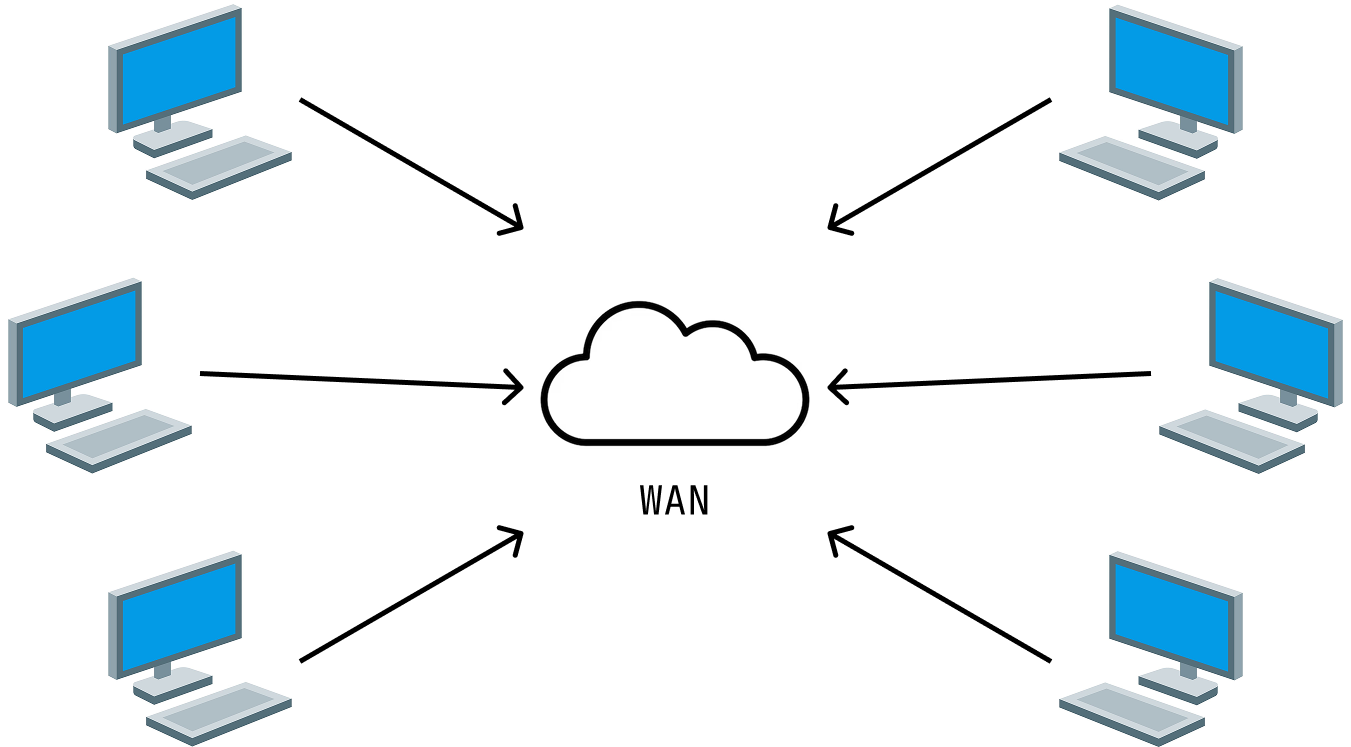
\includegraphics[width=0.5\linewidth]{Images/Protocols/Comunication.png}
    \caption{Comunicazione fra Host}
\end{figure}

\section{Metodologia per comunicare}
La comunicazione, da molto semplice, può diventare complessa. Un modo per nascondere la complessità è l'\textbf{astrazione}. Un modo è dividere l'infrastruttura di rete in diversi \textbf{layer}.

\begin{figure}[!htb]
    \centering
    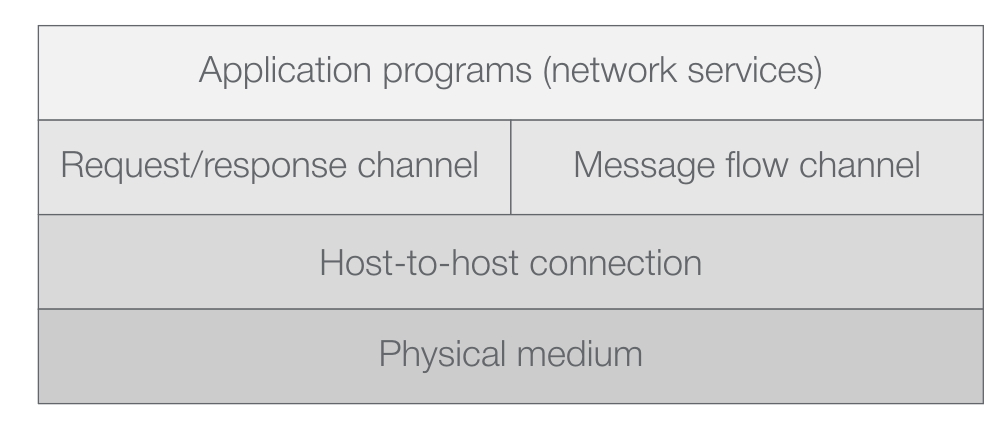
\includegraphics[width=0.6\linewidth]{Images/Protocols/Layers.png}
    \caption{Esempio di layers.}
    \label{fig:layers}
\end{figure}

\newpage
\section{Protocolli}
Le comunicazione richiedono collaborazione e cooperazione per arrivare ad un obiettivo comune, ossia dei \textbf{protocolli} da seguire.

\begin{boxDef}
\textcolor{brown}{\textbf{Protocollo:}} insieme di regole e convenzioni seguite da entità, situate su nodi distinti, che intendono comunicare per svolgere un compito comune.
\end{boxDef}

Ogni protocollo è formato da più parti, tutte utili alla comunicazione:
\begin{enumerate}
    \item \textbf{\textcolor{blue}{Sintassi}:} insieme e strattura di comandi, risposte e formato del messaggio.
    \item \textbf{\textcolor{blue}{Semantica}:} significato dei comandi, delle azione e delle risposte quando trasmetti e ricevi messaggi.
    \item \textbf{\textcolor{blue}{Timing}:} specificazione delle sequenze temporali per comandi, messaggi e risposte.
\end{enumerate}

Comunicazioni complesse richiedono, comunque, l'utilizzo di più protocolli che cooperano fra di loro. I protocolli sono i mattoni di ogni infrastrttura di rete, come l'esempio nella figura \textbf{\ref{fig:layers}}.

Ogni protocollo ha tre interfaccie: 
\begin{enumerate}
    \item Due interfaccie interne per comunicare con il livello superiore e con quello inferiore.
    \item Una interfaccio esterna per comunicare con il protocollo di pari livello di un altro nodo.
\end{enumerate}

\begin{figure}[!htb]
    \centering
    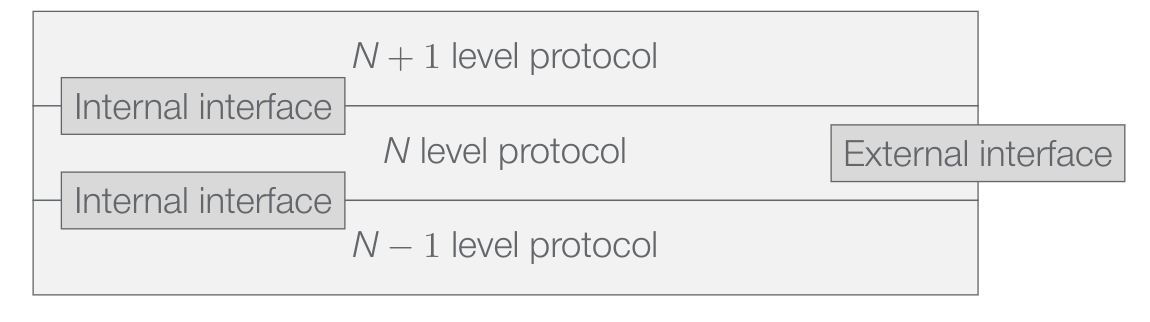
\includegraphics[width=0.6\linewidth]{Images/Protocols/Stack.png}
    \caption{Esempio di comunicazione fra protocolli.}
\end{figure}

\subsection{Protocol Data Unit (PDU)}
Ad ogni livello il messaggio consiste in due parti:
\begin{enumerate}
    \item \textbf{Protocol Control Information (PCI):} ossia l'header.
    \item \textbf{Service Data Unit (SDU):} ossia le informazioni.
\end{enumerate}
L'insieme di queste due parti è il \textbf{PDU}.

\begin{figure}[!htb]
    \centering
    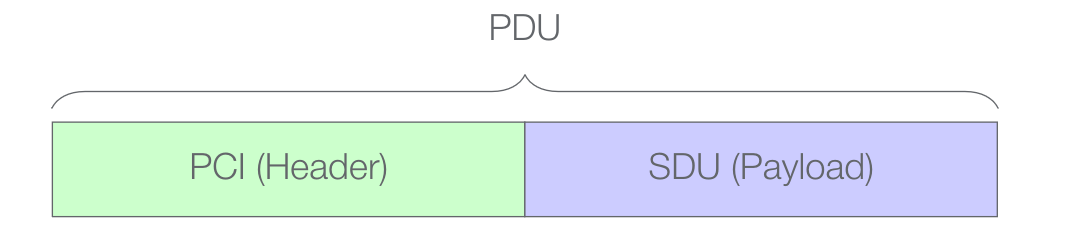
\includegraphics[width=0.6\linewidth]{Images/Protocols/PDU.png}
    \caption{PDU.}
\end{figure}

Ad ogni layer viene incapsulato un header alle informazione, partendo dal livello N fino al livello 1. Successivamente, sarà spacchettato e usato dall'altro host. La gerarchia dei protocolli è definita dall'archittetura dell'infrastruttura di rete a layer.
\chapter{Standard Suite}
Per riuscire a comuninicare fra nodi eterogenei in SW/HW sono necessari degli \textbf{standard}. I due principali sono:
\begin{itemize}
    \item \textbf{\textcolor{red}{ISO-OSI}.}
    \item \textbf{\textcolor{red}{TCP/IP}.}
\end{itemize}

\section{Modello ISO-OSI}
\begin{figure}[!htb]
    \centering
    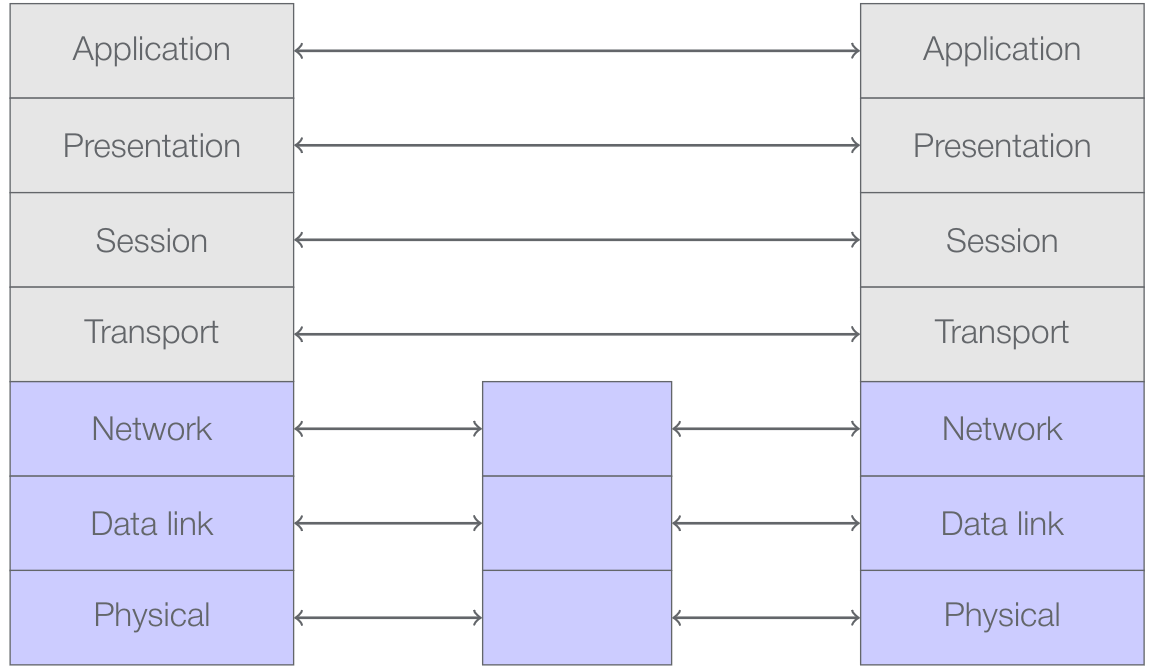
\includegraphics[width=0.6\linewidth]{Images/Standard_Suite/ISO-OSI_Stack.png}
    \caption{ISO-OSI Stack.}
    \label{fig:ISO-OSI}
\end{figure}

\begin{boxDef}
\textcolor{brown}{ISO (International Standard Organization):} defined the specifications of what should have become the protocol standard for the interconnection of heterogeneous nodes.
\\
\vspace*{0.001\textheight}
\\
\textcolor{brown}{OSI (Open Source Informaztion)}
\end{boxDef}

Lo stack \textbf{ISO-OSI} è formato da protocolli di \textbf{elaborazione} per gestire le applicazioni e da protocolli di \textbf{comunicazione} per gestire lo scambio di messaggi fra nodi di rete e per nascondere le caratteristiche del mezzo fisico di trasmissione. Ci sono in totale 7 livelli:
\begin{enumerate}
    \item \textbf{\textcolor{blue}{Fisico.}}
    \item \textbf{\textcolor{blue}{Data-Link.}}
    \item \textbf{\textcolor{blue}{Rete.}}
    \item \textbf{\textcolor{blue}{Trasporto.}}
    \item \textbf{\textcolor{blue}{Sessione.}}
    \item \textbf{\textcolor{blue}{Presentazione.}}
    \item \textbf{\textcolor{blue}{Applicazione.}}
\end{enumerate}

\subsection{Livello Fisico}
Gestisce i dettagli meccanici ed elettrici della trasmissione fisica di un flusso di bit.

\subsection{Livello Data-Link}
Gestisce frame o pacchetti trasformando la semplice trasmissione in una linea di comunicazione priva di errori non rilevati.

\subsection{Livello Rete}
Fornisce connessioni e instradamento dei pacchetti nella rete.

\subsection{Livello Trasporto}
Esegue il controllo end-to-end della sessione di comunicazione, accesso alla rete da parte del client e trasferimento di messaggi tra client.

\subsection{Livello Sessione}
Consente agli utenti su macchine eterogenee di stabilire sessioni, implementando le funzioni di coordinamento, sincronizzazione e mantenimento dello stato.

\subsection{Livello Presentazione}
Risolve le differenze di formato che possono sorgere tra i diversi nodi della rete e gestisce la compressione dei dati, la sicurezza e l'autenticità dei messaggi tramite tecniche di crittografia.

\subsection{Livello Applicazione}
Fornisce un'interfaccia standard per i programmi applicativi che utilizzano la rete, mascherando le peculiarità e la complessità del sistema sottostante.

\subsection{PDU dello stack ISO-OSI}
Ogni livello dello stack ISO-OSI aggiunge un header al PDU, che sarà formato quindi dalla informazioni e 7 header diversi.

\vspace*{0.03\textheight}
\begin{figure}[!htb]
    \centering
    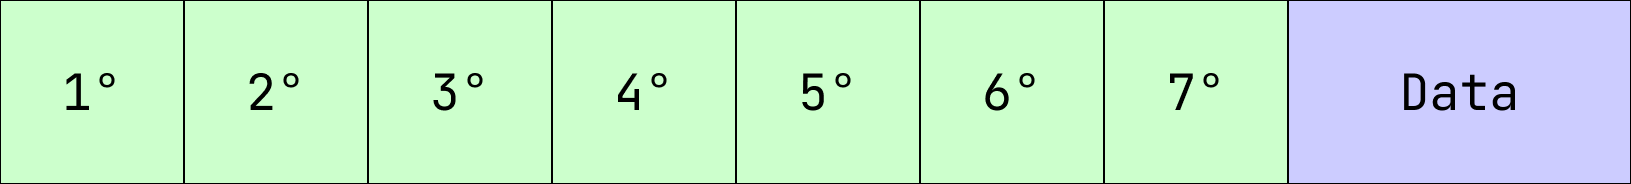
\includegraphics[width=0.7\linewidth]{Images/Standard_Suite/PDU_ISO-OSI.png}
    \caption{ISO-OSI PDU.}
\end{figure}

\newpage
\section{Modello TCP/IP}
\begin{figure}[!htb]
    \centering
    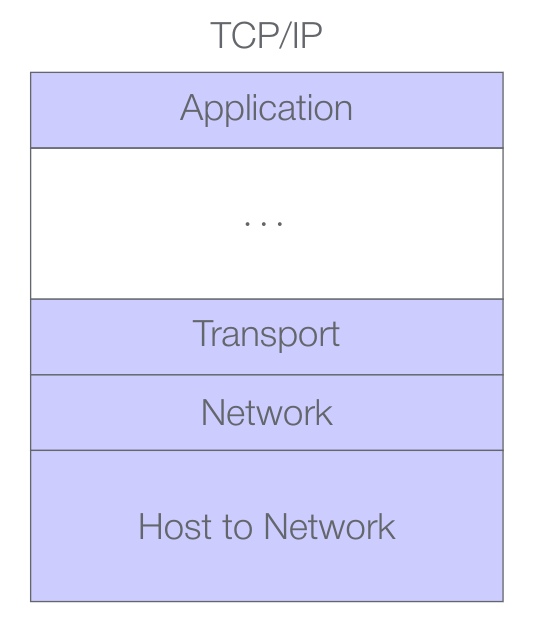
\includegraphics[width=0.3\linewidth]{Images/Standard_Suite/TCP-IP.png}
    \caption{TCP/IP Stack.}
\end{figure}

\textbf{TCP/IP} è il modello più usato ed è di fatto lo standard, anche perchè implementato nei sistemi UNIX e ha molte API per creare applicazione network. 

\subsection{Livello Host-to-Network}
Include i primi due livello del modello ISO-OSI che però rimangono indipendenti. Qui ci sono protoccoli com Ethernet, Token-Ring, 802.11, ecc...

\subsection{Livello Rete}
A questo livello viene usato il protocollo \textbf{IP}, che si occupa di mandare pacchetti dal un nodo sorgente a un nodo destinatario. Tratta ogni pacchetto indipendentemente e non assicura che tutto sia stato inviato correttamente.

\subsection{Livello Trasporto}
Si occupa del multiplezing e demultiplexing dei messaggi fra ogni processo e aggiunge un rilevamento degli errori.
I protocolli principali sono \textbf{TCP} e \textbf{UDP}.

\subsection{Livello Applicazione}
Il livello applicativo utilizza il livello di trasporto delle informazioni tra i processi in esecuzione sugli host terminali per creare applicazioni di rete. Alcuni protocolli usati sono \textbf{SSH}, \textbf{FTP}, \textbf{HTTP}, \textbf{SMTP}, ecc...

\section{Circuit switching}
Un circuito virtuale dedicato per ogni comunicazione, ha la necessità di riservare tutte le risorse end-to-end prima della trasmissione. Risorse dedicate e non è possibile la condivisione.
Ci sono due metodi per dividere le risorse:
\begin{itemize}
    \item \textbf{Frequency Based Methods (FDM).}
    \item \textbf{Time-based methods (TDM).}
\end{itemize}

\section{Packet Switching}
I dati vengono suddivisi in parti e inviati attraverso la rete.
Ogni pacchetto utilizza tutta la capacità di trasmissione di un collegamento. Le risorse vengono utilizzate in base alle necessità e non in base alla prenotazione.
\chapter{Livello Host-to-Network}
\section{Definizione e tecnologie}
Il livello \textbf{H2N} risolve due problemi, quello delle interconnessioni fra due host e quello dello scambio di dati fra due host. Nello specifico il livello \textbf{Fisico} di occupa di connettere gli host con diversi mezzi di trasmissione, invece il livello \textbf{Data-Link} si occupa del framing, del controllo e della correzzione di errori e di inviare i \textbf{\textcolor{blue}{frame}} solo fra nodi della \textbf{LAN}.
Ci sono più tipi di trasmissione:
\begin{enumerate}
    \item \textbf{Broadcast:} comunicazione tra un singolo mittente e tutti gli altri nodi.
    \item \textbf{Multicast:} comunicazione tra un singolo mittente e un gruppo di destinatari.
    \item \textbf{Anycast:} comunicazione tra un singolo mittente e almeno un destinatario in un gruppo.
    \item \textbf{Unicast:} comunicazione tra un singolo mittente e un singolo destinatario.
\end{enumerate}

Il protocollo H2N è implementato nella \textbf{NIC (Netwrok Interface Card)}, tutti i dispositivi della rete per comunicare devono averne una.

\begin{boxDef}
\textbf{\textcolor{brown}{LAN:}} area fisicamente limitate a cui sono connessi uno o più dispotivi. Misurata in \textbf{$\frac{\text{Bit}}{s}$}. Tutte le tecnologie seguono lo standard \textbf{IEEE Standard 802}, come \textbf{Ethernet (IEEE 802.3)} e \textbf{WLAN (IEEE 802.11x)}.
\end{boxDef}

\section{Ethernet}
Creata a metà degli anni '70 da Bob Metcalfe, che propose Ethernet nella sua tesi di dottorato.

\begin{boxDef}
\textcolor{brown}{Ethernet:} metodo di trasmissione usato globalmente perchè economico ed efficente, funziona bene con i protocolli dello stack \textbf{TCP/IP}.
Connessione di tipo \textbf{broadcast}, quindi tutti sono collegati allo stesso canale di comunicazione e anche trasmissione di tipo \textbf{braodcast}, quindi quando viene inviato un messaggio nella \textbf{LAN}, tutti i nodi ad essa collegati lo ricevono.
\end{boxDef}

Gli host utilizzano un indirizzo hardware o indirizzo \textbf{MAC (Media Access Control)} per capire chi è il destinatario dei dati.

\begin{boxDef}
\textcolor{brown}{MAC:} indirizzo unico della \textbf{NIC} a \textbf{48 bit} che viene inserito nella ROM quando viene realizzata. La sua struttura è formata da:
\begin{itemize}
    \item 3 bytes (24 bit) $\rightarrow$ \textbf{Organizationally Unique Identifier (OUI)}, di solito il produttore della NIC.
    \item 3 bytes (24 bit) $\rightarrow$ \textbf{NIC ID}, all'interno dell'OUI.
\end{itemize}
Ogni dispostivo per fare parte della LAN deve avere una NIC e quindi avrà anche un indirizzo MAC unico.
\end{boxDef}

L'indirizzo broadcast è FF-FF-FF-FF-FF-FF.

\newpage
Quindi:
\begin{itemize}
    \item Quando un host desidera trasmettere un pacchetto, inserisce l'indirizzo MAC del destinatario e lo trasmette nella LAN.
    \item Se l'indirizzo di destinazione del pacchetto corrisponde all'indirizzo MAC dell'host ricevente, quest'ultimo accetta il pacchetto e lo inoltra al protocollo successivo.
    \item Se l'indirizzo di destinazione non corrisponde all'indirizzo MAC dell'host ricevente, quest'ultimo scarta il pacchetto.
\end{itemize}

\vspace*{0.02\textheight}
\textbf{ESEMPIO:}
\begin{bashbox}
ddonati@linux > ifconfig eth0
eth0 Link encap:Ethernet HWaddr 00:10:5A:9D:88:AF
inet addr:192.168.1.3 Bcast:192.168.1.255 Mask:255.255.255.0
UP BROADCAST RUNNING MULTICAST MTU:1500 Metric:1
RX packets:92 errors:0 dropped:0 overruns:0 frame:0
TX packets:52 errors:0 dropped:0 overruns:0 carrier:0
collisions:0 txqueuelen:1000
RX bytes:14162 (13.8 KiB) TX bytes:6744 (6.5 KiB)
Interrupt:9 Base address:0xfc00
\end{bashbox}

\textcolor{red}{00:10:5A:9D:88:AF} è l'indirizzo MAC, invece, \textcolor{red}{192.168.1.3} è l'indirizzo IP.

\subsection{Frame Ethernet}
I pacchetti scambiati al livello host to netwrok sono chiamati \textbf{frame}. Per tecnologie e topologie diverse, il formato di ogni frame è sempre lo stesso.

\begin{figure}[!htb]
    \centering
    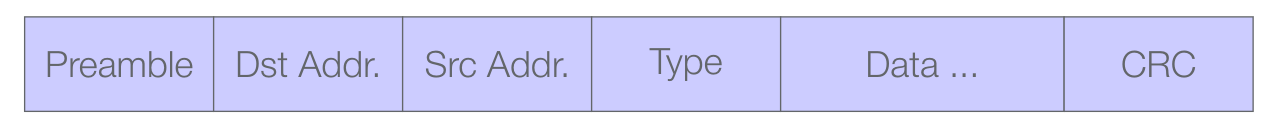
\includegraphics[width=0.9\linewidth]{Images/host_to_network/h2n.png}
    \caption{Frame Ethernet.}
\end{figure}

\subsection{Preamble}
Campo da 8 byte, di cui i primi 7 byte valgono tutti 10101010 e l'ultimo byte vale 10101011. 
I primi 7 byte servono per attivare e sincronizzare i ricevitori, due 1 consecutivi nell'ultimo byte indicano che la sincronizzazione è finita e il contenuto del frame sta per arrivare.

\subsection{Indirizzo di Destinazione e di Origine}
Due campi da 6 byte ciascuno, che indicano l'indirizzo MAC di destinazione e l'indirizzo MAC di origine. Quando un ricevitore riceve un MAC equivalente al suo passa il contenuto al layer di Rete, altrimenti lo scarta.

\subsection{Tipo}
Campo da 2 byte che indica il tipo di protocollo che verrà usato p al layer di Rete (IP, Nevel IPX, Apple Talk, ecc), è usato anche per supportare i protocolli \textbf{ARP} e \textbf{RARP}.

\subsection{Data e Dimensione}
Contiene i dati (\textbf{IP Datagram}), l'unità massima di trasmissione per Ethernet (\textbf{MTU}) è 1500 byte, altrimenti va frammentato, invece, quella minima è 46 byte, se minore di questa cifra va aggiuntoun padding.

\subsection{CRC (Cyclic Redundancy Check)}
Campo da 4 byte che consente all'adattatore che riceve i dati di rilevare la presenza di un errore nei bit del frame ricevuto.

\section{Protocollo ARP}
L'indirizzo IP non è riconosciuto dall'hardware, quindi il protocollo ARP si occupa di trasformare l'IP di un host nella stessa sua LAN nel suo corrispettivo indirizzo MAC.
Nello specifico usa due tipi di messaggi:
\begin{enumerate}
    \item Messaggio broadcast di richiesta con l'indirizzo IP.
    \item Messaggio unicast di risposta con il corrispettivo indirizzo MAC.
\end{enumerate}

\begin{figure}[!htb]
    \centering
    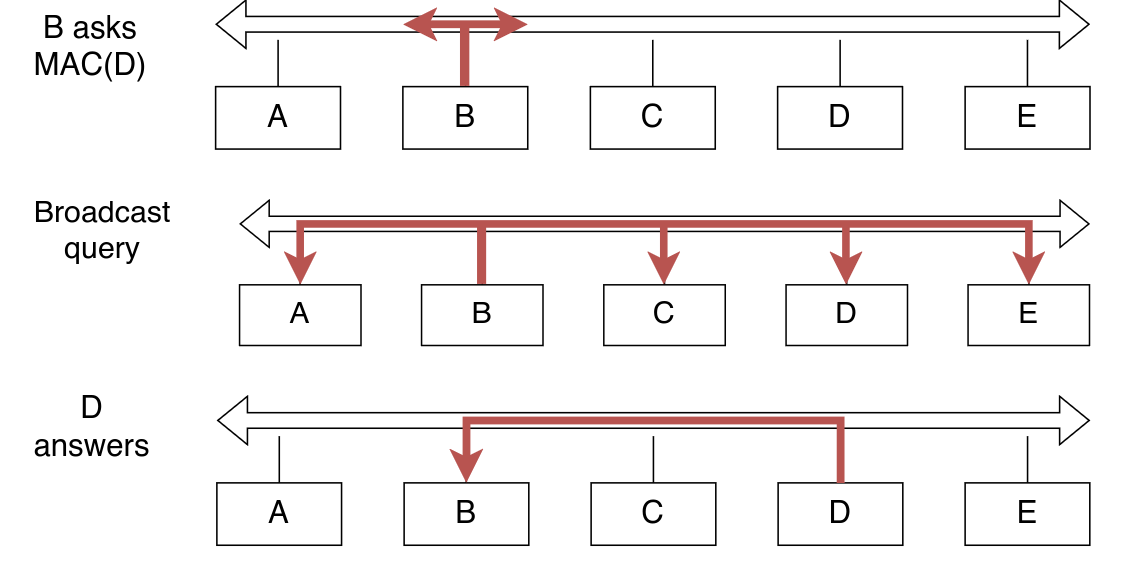
\includegraphics[width=0.7\linewidth]{Images/host_to_network/ARP.png}
    \caption{Protocollo ARP.}
\end{figure}

\subsection{ARP Cache}
Per ridurre il traffico di rete causato dallo scambio di messaggi ARP, ogni host memorizza temporaneamente nella cache le risoluzioni IP/MAC nella propria tabella. 

\begin{center}
\begin{tabular}{ ||c|c|c|| }
 \hline
 \textbf{IP} & \textbf{MAC} & \textbf{TTL} \\ 
 \hline
 \hline
 222.222.222.221 & 88:B2:2F:54:1A:0F & 13:45:00 \\ 
 \hline
 222.222.222.223 & 5C:66:AB:90:75:B1 & 13:52:00 \\ 
 \hline
\end{tabular}
\end{center}

\vspace*{0.02\textheight}
\textbf{ESEMPIO:}
\begin{bashbox}
ddonati@linux > sudo arp
Address HWtype Hwaddress Flags Mask Iface
ns1.ing.unimo.it ether 00:01:03:11:6B:63 C eth0
info-gw.ing.unimo.it ether 00:0A:57:05:A0:00 C eth0

donati@linux > ping brandy.ing.unimo.it
[...]

donati@linux > sudo arp
Address HWtype Hwaddress Flags Mask Iface
brandy.ing.unimo.it ether 00:11:11:5A:EB:41 C eth0
ns1.ing.unimo.it ether 00:01:03:11:6B:63 C eth0
info-gw.ing.unimo.it ether 00:0A:57:05:A0:00 C eth0
\end{bashbox}

\subsection{RARP}
Per ottenere l'indirizzo IP a partire da un indirizzo MAC si può usare il protocollo RARP, che funziona con la stessa struttura e nello stesso modo del protocollo ARP.

\newpage
\section{Interconnessione fra LAN}
Nel fare delle reti LAN molti grandi, possono causarsi molti problemi, dalle collisioni a il limite di lunghezza dello standard 802.3. 
\\
Per questo ci sono diversi tipi di dispositivi di rete, che dipendono da topologia, numero di host connessi, ecc:
\begin{itemize}
    \item \textbf{Hub.}
    \item \textbf{Brigde.}
    \item \textbf{Switch.}
    \item \textbf{L3 Switch.}
\end{itemize}

\subsection{Hub}
Dispositivo di livello fisico con due o più interfacce. Ripete i bit ricevuti su un'interfaccia a tutte le altre interfacce, ogni nodo connesso costituisce un segmento LAN.

\subsection{Bridge}
Dispositivo che opera a livello 2 nell'Ethernet frame, analizza l'header e distribuisce selettivamente in base al MAC di destinazione. Per trasmettere usa il protocollo CSMA/CD.

\subsection{Hub VS Bridge}
Il Bridge è più intelligente di un Hub, dato che è in grado di analizzare gli header e leggere il MAC, quindi, usando delle funzioni da filtro.
Inoltre, è utile perchè elimina le collisioni di dominio, aumenta il throughtput e non necessita di cambiamenti sugli host.
I bridge apprendono quali host sono raggiungibili tramite quali interfacce, infatti:
\begin{enumerate}
    \item Mantengono tabelle di filtro create automaticamente senza la necessità dell'intervento degli amministratori di rete.
    \item Quando viene ricevuto un frame, il bridge apprende la posizione del mittente.
    \item Registra la posizione del mittente nella tabella di filtro usando:
    \begin{itemize}
        \item Indirizzo MAC dell'host.
        \item Interfaccia del bridge.
        \item Time-To-Live (TTL).
    \end{itemize}
\end{enumerate}
I record obsoleti nella tabella di filtro vengono scartati in base alla scadenza del TTL.

\vspace*{0.02\textheight}
\textbf{ESEMPIO:}
\begin{bashbox}
iif frame.destination in filter_table then
    dest_lan_segment = lookup_filter_table(frame.destination)
    forward_to_lan_segment(frame, dest_lan_segment)
else
    {send frame to all ports except incoming port}
    flood(frame)
endif
\end{bashbox}

\subsection{Switch}
Si tratta di bridge ad alte prestazioni con numerose interfacce.
Ci sono più interfacce eterogenee (10/100/1000 Mbps) condivise e dedicate, senza collisioni con accesso dedicato e full duplex.

\subsection{Bridge VS Switch}
Concettualmente sono lo stesso dispositivo, il bridge è software, lo switch è hadrware.

\newpage
\subsection{Brigde in Linux}
\begin{figure}[!htb]
    \centering
    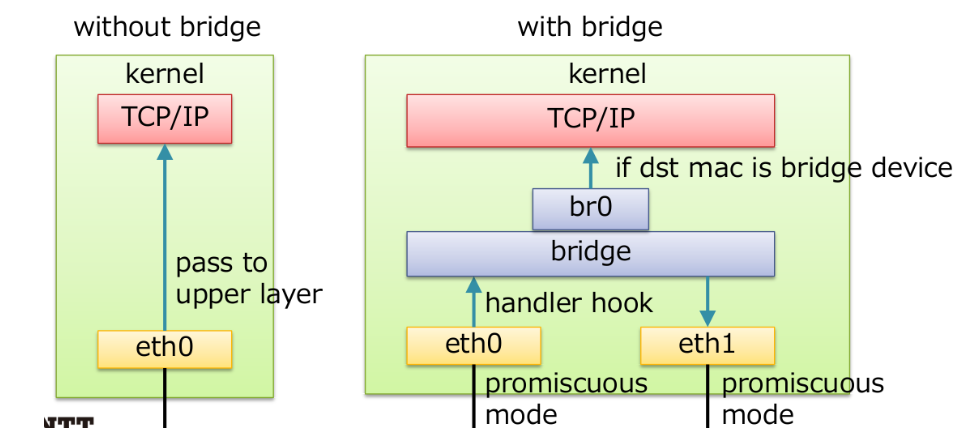
\includegraphics[width=0.7\linewidth]{Images/host_to_network/Bridge.png}
    \caption{Bridge in Linux.}
\end{figure}

I bridge possono essere configurati tramite il file \textbf{/etc/network/interfaces} oppure:

\vspace*{0.02\textheight}
\textbf{Creazione Bridge:}
\begin{bashbox}
bbrctl addbr <bridge>
ip link add <bridge> type bridge ...
\end{bashbox}

\vspace*{0.02\textheight}
\textbf{Aggiungere intefaccie al Bridge:}
\begin{bashbox}
bbrctl addif <bridge> <iface>
ip link set <iface> master <bridge>
\end{bashbox}

\vspace*{0.02\textheight}
\textbf{Vedere i Bridge configurati:}
\begin{bashbox}
bbrctl show <bridge>
\end{bashbox}

\vspace*{0.02\textheight}
\textbf{Vedere la lista dei MAC conosciuti dal Bridge:}
\begin{bashbox}
bbrctl showmacs <bridge>
\end{bashbox}

\newpage
\section{Virtual LAN}
Lo standard 802.1Q definisce le specifiche per definire più reti locali virtuali (VLAN) distinte, utilizzando la stessa infrastruttura fisica. Ogni VLAN agisce come se fosse separata dalle altre:
\begin{itemize}
    \item I pacchetti broadcast sono confinati all'interno della VLAN.
    \item Le comunicazioni a livello 2 sono confinate all'interno della VLAN.
    \item Le VLAN non possono comunicare fra di loro, se non a livello 3 tramite routing.
\end{itemize}
Le VLAN hanno diversi vantaggi tra cui:
\begin{enumerate}
    \item \textcolor{blue}{\textbf{Risparmio:}} evitano di dover creare nuove infrastrutture fisiche.
    \item \textcolor{blue}{\textbf{Performance:}} evita che i frame vengano inviati a destinazioni che non devono riceverli.
    \item \textcolor{blue}{\textbf{Security:}} un utente connesso a una VLAN non ha modo di vedere le altre.
    \item \textcolor{blue}{\textbf{Flessibilità:}} il movimento fisico di un utente non richiede dei cambiamenti fisici ma logici.
\end{enumerate}

Per porter funzionare e quindi riconoscere le VLAN bridge e switch devono essere conformi allo standard 802.1Q.
Devono essere in grado di fare queste tre azioni:
\begin{enumerate}
    \item \textbf{Ingresso:} il bridge deve saper riconoscere a quale VLAN appartiene il frame che arriva da una porta.
    \item \textbf{Trasmissione:} il bridge deve conoscere quale porta il frame deve essere trasmesso, in base alla VLAN alla quale appartiene.
    \item \textbf{Uscita:} il bridge deve essere in grado di far uscire il frame in modo che la sua VLAN venga riconosciuta da altri bridge.
\end{enumerate}
Le Untagged VLAN (private), dove a ogni porta appartiene una VLAN, non richiedono la conformità allo standard 802.1Q, ma solo che lo switch supporti la sua configurabilità.

\subsection{Tagged VLAN}
Lo standard 802.1Q permette di condividere lo stesso accesso fisico e che il bridge sia in grado di riconoscere le varie VLAN. Per questo, sono stati aggiunti 4 byte al frame Ethernet, per speicificare i dati della VLAN:
\begin{itemize}
    \item \textbf{TPI (Tag Protocol Identifier):} due byte, di valore 81 00, che indentifcano il protocollo 802.1Q.
    \item \textbf{TCI (Tag Control Information):} due byte che specificano le informazioni sul tag:
    \begin{itemize}
        \item I primi tre \textbf{(user priority)} indicano la priorità del frame.
        \item Il quarto bit \textbf{(CFI)} se è 1 indica che il frame viene da una token ring LAN.
        \item I restanti dodici bit \textbf{(VID} indica il tag (da 0 a 4095). Il tag 0 e il tag 4095 sono riservati e non possono essere usati.
    \end{itemize}
\end{itemize}

\begin{figure}[!htb]
    \centering
    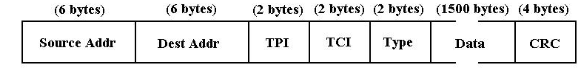
\includegraphics[width=0.7\linewidth]{Images/host_to_network/FrameVLAN.png}
    \caption{Frame standard 802.1Q.}
\end{figure}

\begin{figure}[!htb]
    \centering
    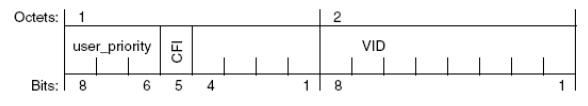
\includegraphics[width=0.7\linewidth]{Images/host_to_network/TCI.png}
    \caption{Campo TCI.}
\end{figure}


\chapter{Livello IP}
\section{Importanza e compiti del livello Netwrok}
Viene definita l'unità di trasferimento dati, ossia il Datagramm (da 64 a 1500 byte). Inoltre, garantisce l'indirizzamento univoco degli host, infatti, tutti gli host connessi a Internet devono essere identificati tramite un Indirizzo IP anche grazie al fatto che viene chiarita l'architettura di Internet. Tutti i router e i sistemi autonomi che compongono Internet possono essere raggiunti tramite funzioni di routing, ossia algoritmi  determinano il percorso dei dati all'interno di una rete geografica. La consegna dei datagrammi però non è affidabile (best-effort).

\begin{figure}[!htb]
    \centering
    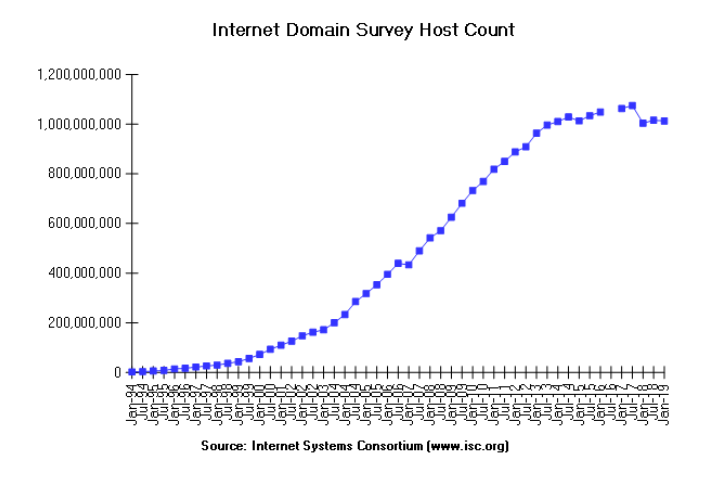
\includegraphics[width=0.7\linewidth]{Images/livello_ip/NumeroIPV4.png}
    \caption{Grafico degli IPv4 unovici su Internet.}
\end{figure}

Non tutti i protocolli a livello Network forniscono un sistema di consegna non affidabile, per esempio la telefonia fornisce un approccio \textbf{connection-oriented}, rispetto all'approccio \textbf{connection-less} di Internet.
Infatti:
\begin{itemize}
    \item \textbf{Circuit Switching:} è necessario riservare tutte le risorse end-to-end prima della trasmissione:
    \begin{itemize}
        \item Non è possibile condividere le risorse assegnate.
        \item Per ogni chiamata è necessaria una fase di configurazione.
        \item Prestazioni garantite in base al tipo di risorse riservate.
    \end{itemize}
    \item \textbf{Packet Switching:} nessuna risorsa riservata:
    \begin{itemize}
        \item Ogni utente può utilizzare tutte le risorse disponibili.
        \item Nessuna configurazione richiesta.
        \item Rischio di conflitti/congestione.
    \end{itemize}
\end{itemize}



\section{Protocollo IP}

\begin{boxDef}
\textcolor{brown}{Protocollo IP:} è un protocollo di comunicazione a livello netwrok, ideato da Vint Cerf e Bob Kahn nel maggio del 1974 e pubblicato sull'IEEE. La prima versione pubblicata è stato IPv4, il suo successore è IPv6.
\end{boxDef}

Il \textbf{protocollo IP} fornisce alcuni servizi molto importanti:
\begin{itemize}
    \item \textbf{Indirizzamento host univoco:} fornisce un grafico praticamente completo di tutti gli host (indirizzi IP).
    \item \textbf{Unità di trasferimento dati:} definisce l'unità di informazione di base utilizzata da Internet per trasferire dati.
    \item \textbf{Funzioni di Routing:} sceglie il percorso nella rete nel quale inviare i pacchetti.
\end{itemize}
La consegna dei pacchetti, però, non è affidabile:
\begin{itemize}
    \item \textbf{Consegna connectionless:} ogni pacchetto è trattato in modo indipendente rispetto agli altri.
    \item \textbf{Consegna Best-Effort:} tentativo di consegnare ogni pacchetto.
    \item \textbf{Consegna non garantita:} i pacchetti possono essere persi, duplicati, ritardati o consegnati fuori ordine.
\end{itemize}

\subsection{Datagram}
\begin{figure}[!htb]
    \centering
    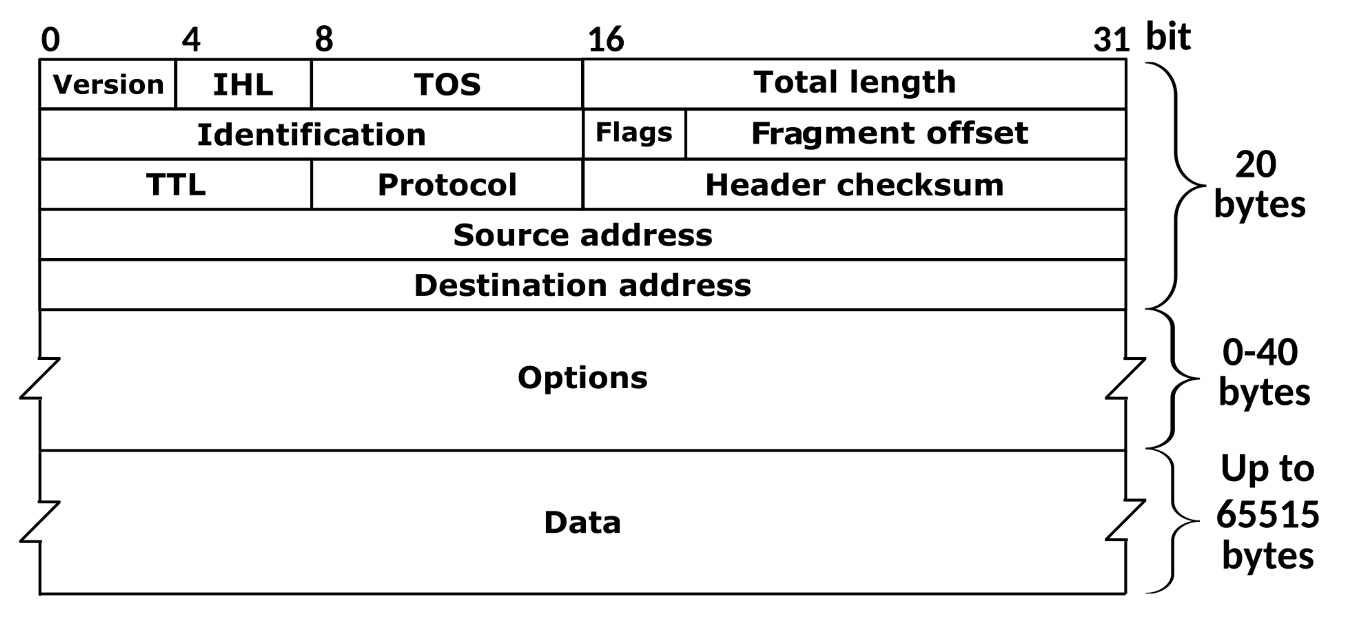
\includegraphics[width=0.9\linewidth]{Images/livello_ip/Datagram.png}
    \caption{Composizione di un Datagram IP.}
\end{figure}

Il \textbf{Datagram IP} è formato da due parti principali, l'header e i dati che effettivamente vengono inviati.
L'header IP a suo volta è formato da diversi campi:
\begin{itemize}
    \item \textbf{Version:} campo da 4 bit con la versione del protocollo IP usato per la creazione del Datagram.
    \item \textbf{IP Header Lenght (IHL):} campo da 4 bit che indica la lunghezza dell'header (massimo 20 byte).
    \item \textbf{Total Lenght:} campo da 16 bit con la lunghezza del Datagram IP (massimo 64kb).
    \item \textbf{Type of Service (TOS):} campo da 8 bit che specifica come il Datagram deve essere trattato, i bit di questo campo sono divisi così:
    \begin{itemize}
        \item \textbf{Precendence:} 3 bit che specificano l'importanza del datagram.
        \item \textbf{Delay (D):} 1 bit.
        \item \textbf{Throughtput (T):} 1 bit.
        \item \textbf{Affidabilità: (R):} 1 bit.
    \end{itemize}
    \item \textbf{Identificazione:} campo da 16 bit che identifica il Datagram.
    \item \textbf{Flags:} controllo della frammentazione:
    \begin{itemize}
        \item \textbf{Reserved.}
        \item \textbf{Don't Fragment (DF).}
        \item \textbf{More Fragment (MF).}
    \end{itemize}
    \item \textbf{Fragment Offset:} indica la posizione del frammento nel datagram originale.
    \item \textbf{Time To Live (TTL):} campo da 8 bit che contiene un contatore (NB: non è un tempo) che indica quanto un datagram può circolare su Internet. Viene decrementato ogni volta che incontra un router e appena arriva a 0 viene eliminato.
    \item \textbf{Protocol:} campo da 8 bit che indica che tipo di protocollo di più alto livello può usare il datagram.
    \item \textbf{Header Checksum:} usato per controllare l'integrità dei dati dell'header del datagram.
    \item \textbf{Indizzo sorgente:} campo da 32 bit con l'indirizzo IP del mandante.
    \item \textbf{Indirizzo di destinazione:} campo da 32 bit con l'indirizzo IP del destinatario.
    \item \textbf{Opzioni:} campo da 32 bit usato per testing e debugging.
    \item \textbf{Padding:} necessario se le opzioni non sono tutte a 32 bit.
\end{itemize}

\section{Ip Addressing}
Ogni indirizzo IPv4 ha 32 bit, diviso in 4 campi da 8 bit ciascuno e seprarati da un punto e sono formati dalla coppia NetID, HostID. Indirizzi nella stessa rete avranno lo stesso NetID ma diverso HostID.

\subsection{Classe di Indirizzi IP}
Per capire quanti bit deve avere il NetID e quanti bit deve avere l'HostID si deve guardare a che classe appartengono:
\begin{itemize}
    \item \textbf{Classe A:} un byte dedicato alla NetID e tre byte dedicati all'HostID. Da 0.0.0.0 a 127.255.255.255.
    \item \textbf{Classe B:} due byte per la NetID e due byte per l'HostID. Da 128.0.0.0 a 191.255.255.255.
    \item \textbf{Classe C:} tre byte per la NetID e un byte per l'HostID. Da 192.0.0.0 a 223.255.255.255.
    \item \textbf{Classe D:} indirizzi multicast riservati. Da 224.0.0.0 a 239.255.255.255. 
    \item \textbf{Classe E:} indirizzi riservati per usi futuri. Da 240.0.0.0 a 255.255.255.254.
\end{itemize}
Ogni IP può essere assegnato dinamicamente o staticammente. Ogni dispositivo può avere più interfacce di rete e quindi avere più IP.
Inoltre, ci sono alcuni indirizzi speciali:
\begin{itemize}
    \item \textbf{Indirizzo della rete:} gli indirizzi con HostID tutto a 0 indicano l'indirizzo della rete.
    \item \textbf{Indirizzo Broadcast:} indirizzi con HostID tutto a 1 funzionano come indirizzo di Broadcast per tutta la rete.
    \item \textbf{Questo Host su questa rete:} l'indirizzo 0.0.0.0 è usato per fare il boot dell'host.
    \item \textbf{Indirizzo di Loopack:} l'indirizzo di classe A con NetID 127 è usato per fare test in locale. Per esempio l'indirizzo Localhost è 127.0.0.1.
\end{itemize}

\section{Subnetting e Supernetting}
La divisione degli indirizzi è molto rigida, per rendere tutto più semplice e maneggevole si possono usare due metodi:
\begin{itemize}
    \item \textbf{Sottoclassi:} per le organizzazioni.
    \item \textbf{Soureclassi:} per gli ISP.
\end{itemize}
Quindi è necessario definire in modo flessibile e logico la coppia \textbf{NetID}, \textbf{HostID}.
Infatti, per definire i bit della NetID viene usata una network mask da 4 byte. Se si fa una operazione di AND fra l'ip e la mask, gli 1 indicheranno la parte dedicata alla NetID e gli 0 indicheranno la parte dedicata all'HostID.

\subsection{Subnetting}
Un'organizzazione può suddividere il proprio spazio di indirizzi host in gruppi chiamati sottoreti:

\begin{figure}[!htb]
    \centering
    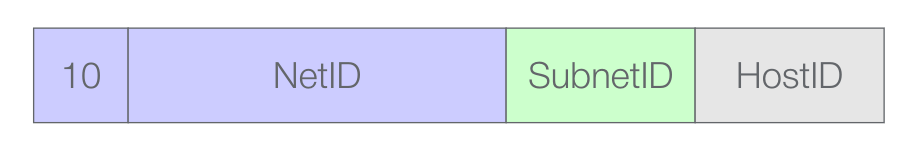
\includegraphics[width=0.7\linewidth]{Images/livello_ip/Subnet.png}
    \caption{Esempio di indirizzo di una subnet.}
\end{figure}

\textbf{ESEMPIO:}
\begin{boxDef}
Dati:
\begin{itemize}
    \item \textbf{IP address:} 192.168.81.56
    \item \textbf{Netmask:} 255.255.255.240
\end{itemize}

Per calcolare il NetID: 
\\
IP Address \textbf{10011100.10011010.01010001.00111000} = \textbf{156.154.81.56}
\\
Netmask \textbf{11111111.11111111.11111111.11110000} = \textbf{255.255.255.240}
\\
Result \textbf{10011100.10011010.01010001.00110000} = \textbf{156.154.81.48}
\end{boxDef}

\section{Architettura di Internet}
Internet non è un insieme di router sparsi a caso per il mondo che sono interconnessi tra loro.
\begin{boxDef}
\textbf{\textcolor{brown}{Internet:}} la definizione di \textbf{Internet} dipende dal punto di vista:
\begin{itemize}
    \item Dal punto di vista delle \textbf{applicazioni di rete}, ossia un'entità trasparente, nella maggior parte dei casi.
    \item Dal punto di vista \textbf{fisico}, un insieme di componenti interni, in cui ogni nodo è caratterizzato da un indirizzo IP.
    \item Dal punto di vista \textbf{organizzativo}, un insieme di sistemi autonomi (considerando i \textbf{router}) e un insieme di nomi e domini (considerando gli \textbf{host}).
\end{itemize}
\end{boxDef}

Ha alcuni principi:
\begin{itemize}
    \item \textbf{Sopravvivenza:} se esiste un percorso tra i due host, la comunicazione deve essere in grado di continuare.
    \item \textbf{Forma a clessidra:} IP fa ipotesi minime sui mezzi di trasferimento dati sottostanti. Deve funzionare per tutti i tipi di applicazioni di rete e con un approccio senza stato.
    \item \textbf{Sistemi autonomi:} ogni rete è di proprietà e gestita da un'entità diversa.
\end{itemize}

\subsection{Autonomous System}
\begin{boxDef}
\textbf{\textcolor{brown}{AS:}} un insieme di \textbf{reti IP} e \textbf{router} sotto il controllo di un'organizzazione all'interno della quale viene utilizzata una politica di \textbf{routing} interna. Tutti i router all'interno dello stesso \textbf{AS} utilizzano lo stesso algoritmo di instradamento dei messaggi e si scambiano continuamente informazioni con gli altri router.
Dall'esterno, i \textbf{sistemi autonomi} sono visti come un'unica entità.
\end{boxDef}
Gli AS sono interconnessi fra di loro in due modi:
\begin{enumerate}
    \item Attraverso punti di peering privati.
    \item Attraverso punti di scambio Internet (IXP).
\end{enumerate}

\section{Routing}
Inoltrare pacchetti all'interno di una rete è un problema complesso, per questo si può dividere in sottoproblemi:
\begin{enumerate}
    \item Ad ogni hop, inoltra il pacchetto a un altro nodo in modo che si avvicini alla destinazione (IP forwarding).
    \item Mantenere le informazioni aggiornate per poter risolvere il primo sottoproblema (Gestione delle tabelle di routing).
\end{enumerate}

\begin{boxDef}
\textbf{\textcolor{brown}{IP Forwarding:}} operazione eseguita da ogni \textbf{router}. Il router successivo deve appartenere alla \textbf{rete} a cui il router è direttamente connesso. Per inoltrare i pacchetti, l'indirizzo di destinazione viene estratto dall'header del \textbf{pacchetto} e viene utilizzato come indice nella tabella di routing.
\end{boxDef}
L'IP forwarding ha alcune caratteristiche importanti:
\begin{itemize}
    \item \textbf{Indipendenza dal mittente:} il routing del next-hop non dipende dal mittente del pacchetto o dal percorso che il pacchetto ha percorso fino a quel punto.
    \item \textbf{Routing universale:} la tabella di routing deve contenere un router next-hop per ogni destinazione.
    \item \textbf{Routing ottimale:} il router next-hop viene scelto in modo da minimizzare il percorso verso la destinazione con l'utilizzo di algoritmi di routing.
\end{itemize}

\begin{boxDef}
\textbf{\textcolor{brown}{Tabelle di Routing:}} ogni host e ogni router possiede una tabella di routing. Ogni riga indica il next-hop per ogni possibile destinazione.
\end{boxDef}

Esistono due tipi di \textbf{Routing}:
\begin{enumerate}
    \item \textbf{Statico:} 
    \begin{itemize}
        \item La tabella di routing non viene modificata dal router.
        \item L'amministratore di rete deve inserire o modificare le righe della tabella di routing.
        \item Impossibilità di reagire automaticamente ai cambiamenti topologici.
        \item Da utilizzare in caso di reti di piccole dimensioni con poche modifiche.
    \end{itemize}
    \item \textbf{Dinamico:}
    \begin{itemize}
        \item La tabella di routing viene modificata dal router al variare delle condizioni di rete.
        \item Lo scambio di informazioni e il calcolo dei valori della tabella di routing avvengono tramite protocolli di routing.
    \end{itemize}
\end{enumerate}

\vspace*{0.02\textheight}
\textbf{ESEMPIO DI IP FORWARDING:}
\begin{figure}[!htb]
    \centering
    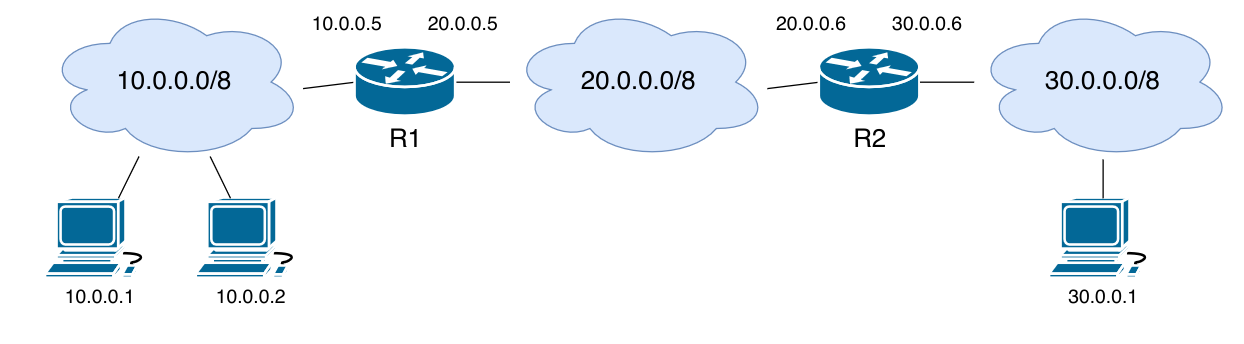
\includegraphics[width=0.8\linewidth]{Images/livello_ip/IPForwarding.png}
    \caption{Esempio di indirizzo di una subnet.}
\end{figure}

Si hanno queste tabelle di routing per quanto riguarda i router:
\begin{center}
    \begin{minipage}{.4\textwidth}
        \begin{tabular}{ || c | c ||}
            \hline
            \textbf{DESTIONATION} & \textbf{NEXT HOP} \\
            \hline
            \hline
            10.0.0.0/8 & direct \\
            \hline
            20.0.0.0/8 & direct \\
            \hline
            30.0.0.0/8 & 20.0.0.6 \\
            \hline
        \end{tabular}
    \end{minipage}
    \begin{minipage}{.4\textwidth}
        \begin{tabular}{ || c | c ||}
            \hline
            \textbf{DESTIONATION} & \textbf{NEXT HOP} \\
            \hline 
            \hline
            10.0.0.0/8 & 20.0.0.5 \\
            \hline
            20.0.0.0/8 & direct \\
            \hline
            30.0.0.0/8 & direct \\
            \hline
        \end{tabular}
    \end{minipage}
\end{center}

E queste tabelle di routing per quanto riguarda gli host:
\begin{center}
    \begin{minipage}{.4\textwidth}
        \begin{tabular}{ || c | c || }
            \hline
            \textbf{DESTIONATION} & \textbf{NEXT HOP} \\
            \hline
            \hline
            10.0.0.0/8 & direct \\
            \hline
            default & 10.0.0.5 \\
            \hline
        \end{tabular}
    \end{minipage}
    \begin{minipage}{.4\textwidth}
        \begin{tabular}{ || c | c || }
            \hline
            \textbf{DESTIONATION} & \textbf{NEXT HOP} \\
            \hline
            \hline
            10.0.0.0/8 & direct \\
            \hline
            default & 30.0.0.6 \\
            \hline
        \end{tabular}
        \label{Tabella di Routing di 30.0.0.1}
    \end{minipage}
\end{center}

\vspace*{0.02\textheight}
Se volessi mandare un pacchetto dall'host \textbf{10.0.0.1} all'host \textbf{10.0.0.2} sarebbe necessario solamente il protocollo ARP, invece, se volessi mandare un pacchetto dallo stesso host sorgente all'host \textbf{30.0.0.1}, dovrei passare prima per il router R1 (sempre tramite il protocollo ARP) e successivamente andare al router R2 per raggiungere l'host di destinazione.

\subsection{Teoria del Routing}
L'obiettivo del routing è stabilire il percorso ottimale, ossia quello con costo minore che colleghi i due host che vogliono comunicare.
Per formulare un algoritmo di routing, la rete viene modellata utilizzando un grafo pesato \textbf{G(N, E)} dove:
\begin{itemize}
    \item I nodi \textbf{N} rappresentano i router (o gli AS).
    \item Gli archi \textbf{E} rappresentano le connessioni tra i router.
    \item Le etichette degli archi \textbf{E} rappresentano il "costo" delle connessioni tra i router.
\end{itemize}
Si dividono in due categorie principali:
\begin{enumerate}
    \item \textbf{Algoritmi di routing distribuiti}:nessun nodo possiede informazioni complete sul costo di tutti i collegamenti nella rete.
    \item \textbf{Algoritmi di routing centralizzati:} ogni nodo possiede informazioni globali sulla rete.
\end{enumerate}

\begin{figure}[!htb]
    \centering
    
\includegraphics[width=0.5\linewidth]{Images/livello_ip/Grafo.png}
    \caption{Grafo pesato.}
\end{figure}

Ci sono alcuni fattori che possono influenzare il routing, come la topologia, traffico, fallimenti e policies.

\newpage
\subsection{Distan Vector Protocol}
Calcolo \textbf{distribuito} del \textbf{next hop}, è un algoritmo adattivo rispetto ai cambiamenti di stato. Esempio di implementazione principale è l'algoritmo distribuito di Bellman-Ford.

\subsubsection{Algortimo di Bellman-Ford}
Compiti di ciascun nodo:
\begin{itemize}
    \item Aggiornamento del vettore di distanza in risposta alle variazioni di costo sui collegamenti adiacenti.
    \item Invio di un aggiornamento ai nodi adiacenti se il loro vettore di distanza cambia.
\end{itemize}
Dati su ciascun nodo \textbf{x}:
\begin{itemize}
    \item $c(x, v)$ costo del collegamento tra il nodo \textbf{x} e il nodo vicino \textbf{v $\in$ V}.
    \item \textbf{Dx} = \{$Dx(y)$ : y $\in$ N\} vettore delle distanze dal nodo x a tutti i nodi \textbf{y} $\in$ rete \textbf{N}.
    \item \textbf{Dv} = \{$Dv(y)$ : y $\in$ N\} vettori di distanza dei nodi vicini \textbf{v} $\in$ \textbf{V} di \textbf{x}.
\end{itemize}
Bellman-Ford serve per calcolare il costo minimo da \textbf{x} a \textbf{y}: 
\[
Dx(y) = min_v\{c(x, v) + Dv(y)\}
\]
Dove $min_v$ è calcolato su tutti i nodi \textbf{v} vicini al nodo \textbf{x}. Tra tutti i nodi \textbf{v} adiacenti al nodo \textbf{x}, il percorso da scegliere è quello che porta da \textbf{v} a \textbf{y} con il costo più basso.

\vspace*{0.02\textheight}
\textbf{INIZALIZZAZIONE:}
\begin{bashbox}
ffor all y in N do
    if y in V then
        Dx(y) = c(x, y)
    else
        Dx(y) = infinito

    Send vector Dx to all v in V
\end{bashbox}

\textbf{LOOP:}
\begin{bashbox}
while True do
    # Wait for change in neighbor link cost or update
    for all y in N do
        Dx(y) = minv{c(x, v) + Dv(y)}
        
        if exist y in N : Dx(y) changed then
            Send vector Dx to all v in V
\end{bashbox}

\begin{figure}[!htb]
    \centering
    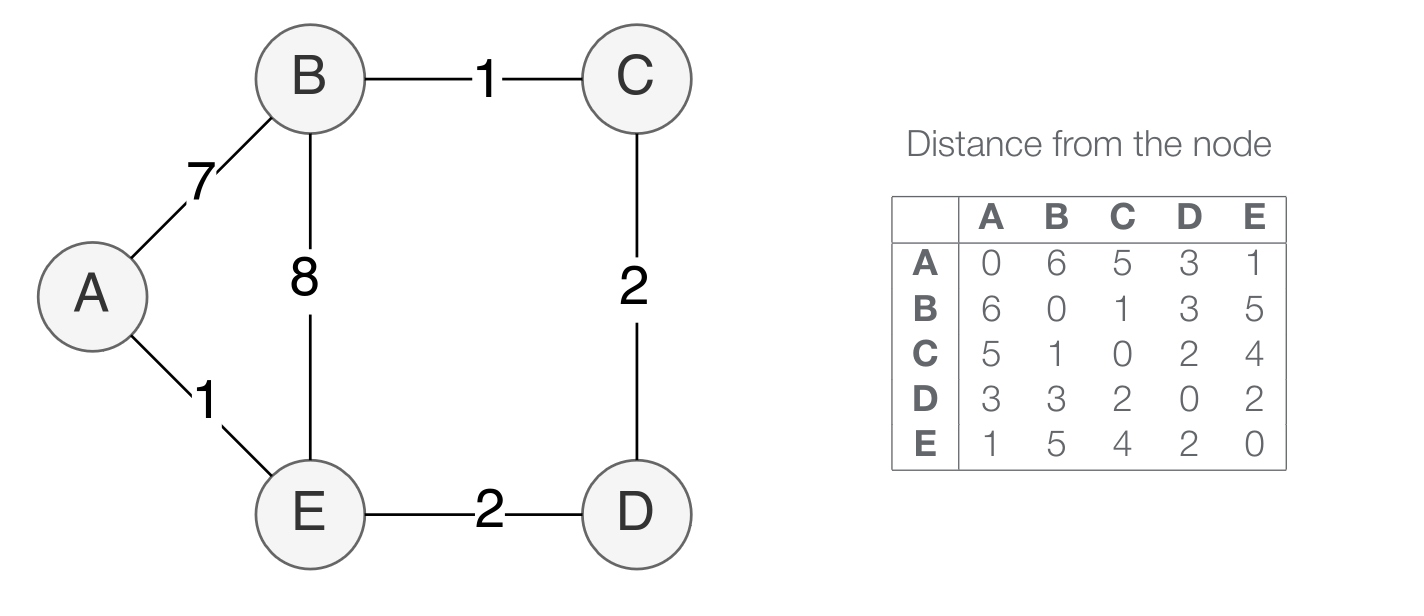
\includegraphics[width=0.7\linewidth]{Images/livello_ip/Bellman-Ford.png}
    \caption{Esempio di tabella di Routing con Bellman-Ford.}
\end{figure}

\subsection{Problemi}
Se il costo di un percorso aumenta e il percorso alternativo minimo contiene il percorso che è aumentato, il pacchetto non arriverà ma a destinazione ma farà avanti e indietro. Questo è chiamato \textbf{Rebound Effect}. Se un nodo è connesso tramite un collegamento e il collegamento si guasta, allora non si avrà stabilizzazione e si avrà un problema \textbf{Count-to-Infinity}.
\\
Le possibili soluzioni sono tre:
\begin{enumerate}
    \item Scegliere un \textbf{threeshold} per rappresentare il valore "infinito".
    \item \textbf{Split Horizon:} è necessario differenziare i vettori di distanza inviati ai nodi adiacenti. Il vettore di B inviato a C non conterrà le destinazioni raggiungibili tramite C.
    \item \textbf{Split Horizon with poisoned reverse:} se B raggiunge A passando per C, B avvertirà C che la sua distanza da A è infinita.
\end{enumerate}

\subsection{Algoritmi Link State}
Sono algoritmi \textbf{centralizzati}, necessitano di conoscere la \textbf{topologia} e il \textbf{costo} di ogni collegamento. Tutti i nodi hanno una visione identica e completa della rete e fanno diverse cose:
\begin{enumerate}
    \item Calcolano lo stato dei loro collegamenti.
    \item Trasmettono periodicamente l'identità e i costi dei loro collegamenti connessi.
    \item Calcolano i percorsi a costo minimo verso tutti gli altri nodi della rete utilizzando l'algoritmo di Dijkstra.
\end{enumerate}
Tutte queste informazioni sono contenute nel \textbf{Link State Packet}, nello specifico: 
\begin{itemize}
    \item Node ID.
    \item Lista dei vicini e costi dei collegamenti.
    \item Time To Live (TTL).
    \item Sequence Number per riconoscere eventuali errori.
\end{itemize}

\vspace*{0.02\textheight}
\textbf{PROPAGAZIONE DEI PACCHETTI:}
\begin{bashbox}
iif P is most recent packet form j then
    save P to database
    for all links != incoming link of P do
        Forward P
    else
        Discard P
\end{bashbox}

\subsubsection{Algortimo di Dijkstra}
Algoritmo iterativo, quindi, all'iterazione k, il nodo i conosce il percorso a costo minimo verso k nodi di destinazione. Abbiamo: 
\begin{itemize}
    \item $c(i, j)$ costo del collegamento tra il nodo \textbf{i} e il nodo \textbf{j}.
    \item $D(v)$ costo minimo del percorso verso il nodo \textbf{v} (minimo per l'iterazione corrente).
    \item $p(v)$ predecessore immediato di \textbf{v} lungo il percorso a costo minimo verso \textbf{v}.
    \item \textbf{N} gruppo di nodi il cui percorso a costo minimo è definitivamente noto.
\end{itemize}

\vspace*{0.01\textheight}
\textbf{INIZIALIZZAZIONE:}
\begin{bashbox}
NN = {u}
for all nodes v do
    if v is adjacent to u then
        D(v) = c(u, v)
    else
        D(v) = infinito
\end{bashbox}

\textbf{LOOP:}
\begin{bashbox}
rrepeat
    #Compute for all adjacent nodes i not in N the cost D(i)
    Add to N the node w with the minimum cost D(w)
    for all Nodes v adjacent to w and not in N do
        # new cost to v is the old one or the lowest cost to w plus the cost from w to v
        D(v) = min{D(v), D(w) + c(w, v)}
until all the nodes of the graph in N
\end{bashbox}

\begin{figure}[!htb]
    \centering
    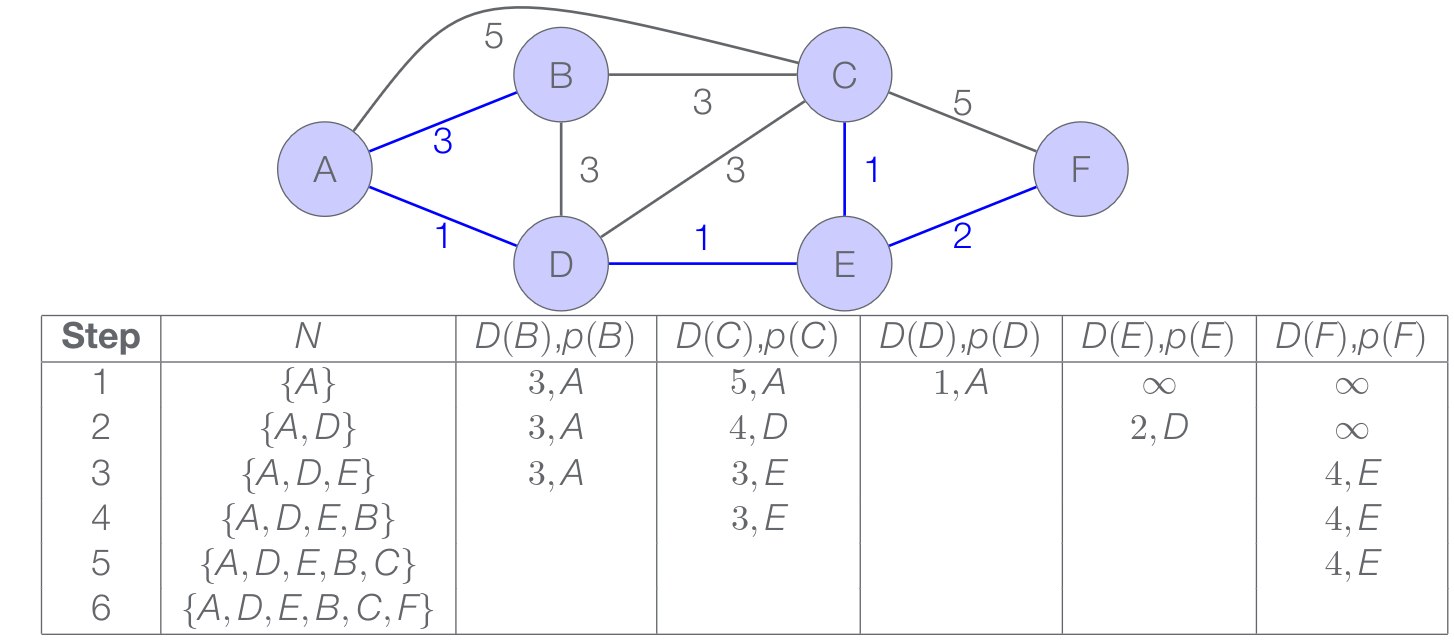
\includegraphics[width=0.8\linewidth]{Images/livello_ip/Dijkstra.png}
    \caption{Esempio di tabella di Routing con Dijkstra.}
\end{figure}

\subsection{Differenze fra Distan Vector Protocol e Algortimi Link State}
Non ci sono algoritmi migliori di altri, gli algortimi \textbf{Link State} sono usati spesso all'interno degli \textbf{AS}, invece, i \textbf{Distant Vector Algoritm} sono più usati fra \textbf{AS}.
\begin{center}
    \begin{minipage}{.45\linewidth}
        \begin{boxDef}
        \textbf{\textcolor{brown}{Distan Vector Protocol:}}
            \begin{itemize}
                \item Tutto ciò che è noto viene propagato solo ai vicini.
                \item Messaggi potenzialmente molto larghi.
                \item Numero di messaggi piccolo.
                \item Lenta convergenza e rischio di Rebound Effect o delay elevati.
                \item Requisiti di memoria piccoli.
                \item Calcoli del router basati su calcoli di altri router.
            \end{itemize}
        \end{boxDef}
    \end{minipage}
    \begin{minipage}{.45\linewidth}
        \begin{boxDef}
        \textbf{\textcolor{brown}{Algoritmi Link State:}}
            \begin{itemize}
                \item Le informazioni sono passate a tutti.
                \item Messaggi piccoli.
                \item Numero elevato di messaggi ($O(n)$ dove $n$ è il numero di nodi del grafo).
                \item Convergenza molto veloce.
                \item Requisiti di memoria elevati.
                \item Ogni router calcoli la route del percorso indipendentemente.
            \end{itemize}
        \end{boxDef}
    \end{minipage}
\end{center}

\newpage
\section{Routing a scala geografica}
Ogni \textbf{AS} ha un numero di identificazione, compreso tra 1 e 64511, assegnato da un'autorità di registrazione \textbf{Internet}. I numeri tra 64512 e 65535 sono riservati.
\\
Per il routing dentro gli AS (\textbf{Intra-AS routing}) si usa un \textbf{Interior Gateway Protocol}, cioè i router di un AS possono avere informazioni complete su tutti gli altri router dell'AS.
Per il routing fra AS (\textbf{Inter-AS routing}) si usa un \textbf{External Gateway Protocol}.
\\
Esistono diversi tipi di AS:
\begin{itemize}
    \item \textbf{Stub:} AS con una sola connessione a un altro AS.
    \item \textbf{Multi-Homed:} un AS è connesso con diversi altri AS, ma accetta solo traffico locale.
    \item \textbf{Transit:} un AS connesso a diversi AS che possono fungere da intermediari per l'AS a cui è connesso.
\end{itemize}
I protocolli di routing principali sono:
\begin{itemize}
    \item \textbf{Border Gateway Protocol (BGP)} per il routing \textbf{Inter-AS}.
    \item \textbf{Routing Information Protocol (RIP)} per il routing \textbf{Intra-AS}, come \textbf{Distance Vector Protocol}, non più usato.
    \item \textbf{Open Shortest Path First (OSPF)} per il routing \textbf{Intra-AS}, come \textbf{Link State Protocol}, quello che viene usato ora.
\end{itemize}

\subsection{Border Gateway Protocol (BGP)}
Protocollo delle backbones di Internet usato da ISP per gestire il traffico tra i sistemi autonomi in modo completamente decentralizzato. Ha alcune funzioni principali:
\begin{itemize}
    \item Scambio di informazioni di raggiungibilità tra AS vicini, chiamati \textbf{peer}.
    \item Propaga le informazioni di raggiungibilità a tutti i router all'interno di un AS con un meccanismo distribuito basato sull'algoritmo \textbf{Path Vector}.
    \item Determina i percorsi migliori in base alle informazioni di raggiungibilità e alle \textbf{politiche di instradamento}.
\end{itemize}
Per comunicare vengono utilizzate connessioni TCP semi-permanenti per consentire ai router vicini di comunicare, creando di fatto una \textbf{sessione} BGP. Le sessioni possono essere di due tipi: 
\begin{enumerate}
    \item \textbf{External session (E-BGP)} fra router (\textbf{Border Router)} di diversi AS.
    \item \textbf{Internal session (I-BGP} fra router (Transit Router) dello stesso AS.
\end{enumerate}

\begin{figure}[!htb]
    \centering
    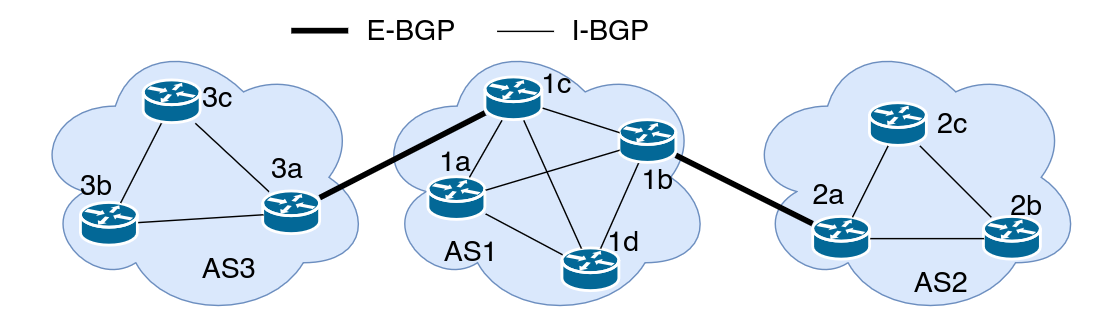
\includegraphics[width=0.8\linewidth]{Images/livello_ip/BGP.png}
    \caption{Routing BGP.}
\end{figure}

\subsubsection{Algoritmo Path Vector}
BGP utilizza Path Vector, una variante dell'algoritmo distribuito Distance Vector Protocol. Ogni aggiornamento di routing contiene non solo informazioni adiacenti, ma anche informazioni sull'intero percorso verso la destinazione tramite gli AS. Utilizza metriche e politiche locali nei processi decisionali e garantisce l'assenza di cicli.

\newpage
\subsection{Open Short Path First (OSPF)}
Il routing si basa sull'algoritmo centralizzato \textbf{Link State}. La topologia e costi noti a ciascun nodo, l'albero del percorso a costo minimo viene calcolato utilizzando l'algoritmo di \textbf{Dikstra} e memorizzato nel cosiddetto "database di stato dei collegamenti", distribuito a tutti i router periodicamente. Gli aggiornamenti, invece, vengono trasmessi in broadcast ai router dell'intero AS (\textbf{flooding}) direttamente su \textbf{IP}.
Le funzionalità principali sono: 
\begin{itemize}
    \item \textbf{Sicurezza:} autenticazione dei messaggi OSPF con algoritmi di crittografia.
    \item \textbf{Percorsi multipli con costo uguale:} possibilità di utilizzare percorsi multipli per instradare il traffico.
    \item \textbf{Supporto integrato per il routing unicast e multicast:} multicast OPSF (\textbf{MOSPF}) utilizza lo stesso database di collegamenti di OSPF.
    \item \textbf{Struttura gerarchica degli AS:} possibilità di strutturare grandi domini di routing in gerarchie di AS.
\end{itemize}

\subsection{Struttura di un messaggio OSPF}
Formato da un header in comune e un body che dipende dal tipo. \\
\begin{figure}[!htb]
    \centering
    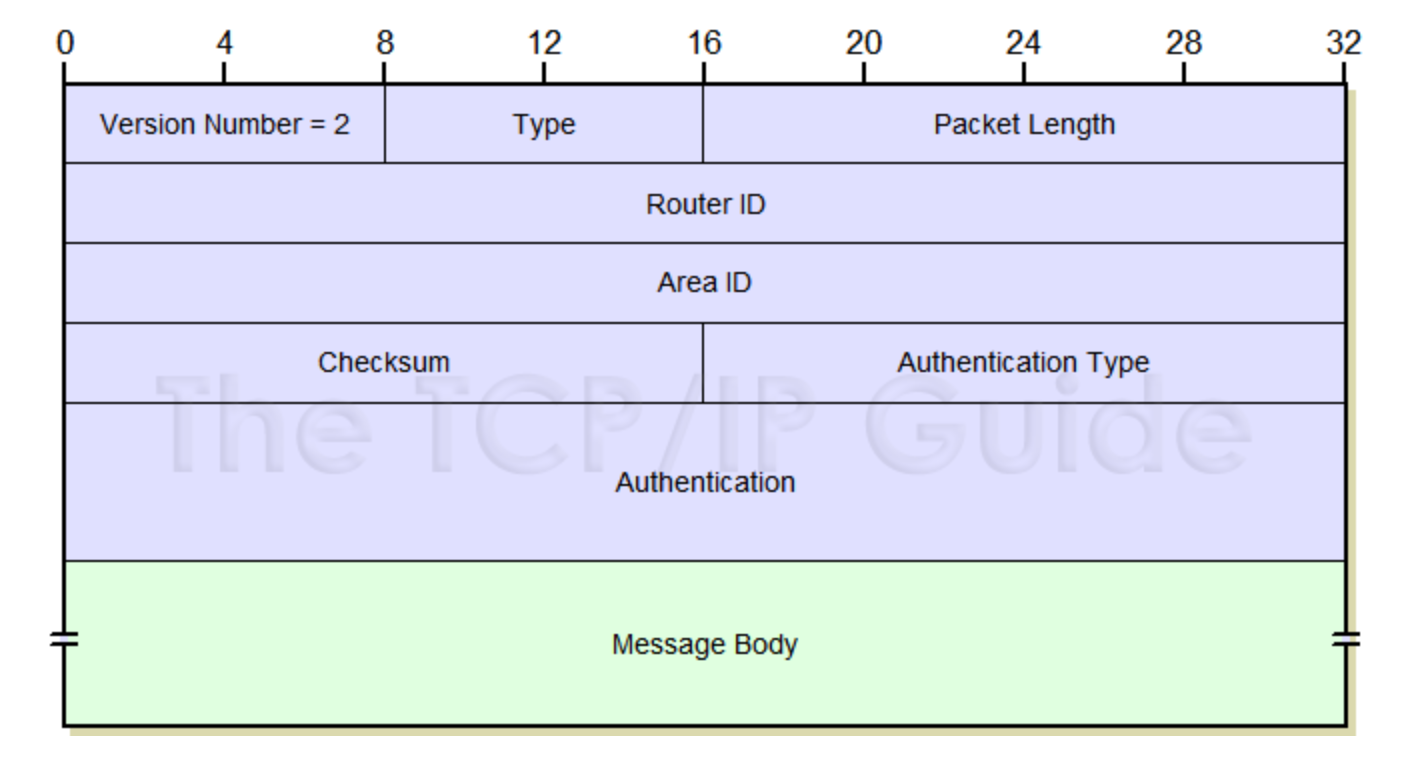
\includegraphics[width=0.70\linewidth]{Images/livello_ip/OSPF.png}
    \caption{Messaggio con OSPF.}
\end{figure}
L'header è formato da:
\begin{itemize}
    \item \textbf{Versione number.}
    \item \textbf{Tipo:}
    \begin{itemize}
        \item Hello.
        \item DB Description.
        \item Link State Req.
        \item Link State Update.
        \item Link State ACK.
    \end{itemize}
    \item \textbf{Dimensione:} misurata in byte (header + body).
    \item \textbf{Router ID:} ip dell'interfaccia da dove è inviato il messaggio.
    \item \textbf{AreaID:} area a cui il messaggio appartiene.
    \item \textbf{Checksum:} include tutto tranne che i campi di autenticazione.
    \item \textbf{Tipo di autenticazione:} può essere 0 (niente), 1 (con password) e 2 (crittografata).
    \item \textbf{Informazioni di autenticazione.}
\end{itemize}

\subsection{Struttura della gerarchia OSPF}
Consente di suddividere i grandi sistemi autonomi (AS) in aree in modo da avere una gerarchia interna a due livelli:
\begin{itemize}
    \item \textbf{Aree locali:} comunicano le rotte verso altre aree locali del sistema autonomo ai router di tali aree.
    \item \textbf{Aree Backbone:} instrada il traffico tra le aree del sistema autonomo, contiene tutti i border router.
\end{itemize} 
L'algoritmo Link State viene utilizzato all'interno di ciascuna area.

\section{IPv6}

\chapter{Livello Trasporto}
\section{Introduzione}
Il livello di trasporto estende il servizio di consegna del protocollo IP tra due host terminali a un servizio di consegna per due processi applicativi in esecuzione sugli host.
Inoltre, aggiunge alcune funzionalità, come il controllo di errori e il multiplexing/demultiplexing dei messaggi fra processi.
I protocolli principali sono due:
\begin{enumerate}
    \item \textbf{TCP (Trasmission Control Protocol).}
    \item \textbf{UDP (User Datagram Procotol).}
\end{enumerate}

\begin{figure}[!htb]
    \centering
    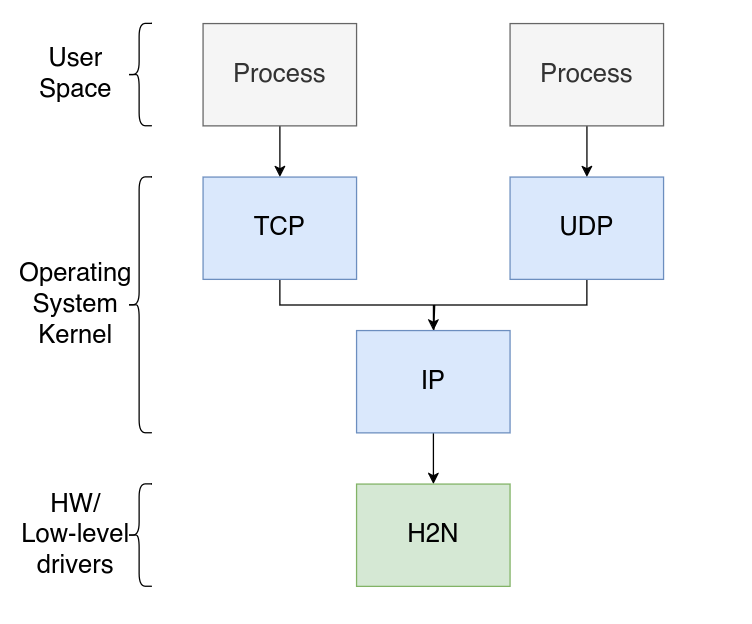
\includegraphics[width=0.5\linewidth]{Images/livello_trasporto/Trasporto.png}
    \caption{Schema comunicazione con protocolli e livelli.}
\end{figure}

\subsection{Multiplexing e Demultiplexing}
Il protocollo IP non trasferisce dati tra i processi applicativi in esecuzione sui nodi finali, questo è compito dei protocolli di trasporto:
\begin{itemize}
    \item \textbf{Multiplexing:} creazione di segmenti derivanti da messaggi di diversi processi applicativi, avviene sul nodo sorgente.
    \item \textbf{Demultiplexing:} ogni segmento del livello di trasporto ha un campo contenente le informazioni utilizzate per determinare a quale processo il segmento deve essere consegnato, avviene del nodo di destinazione.
\end{itemize}
I protoclli UDP e TCP aggiungo per fare questo due campi nell'header del segmento:
\begin{enumerate}
    \item \textbf{Numero di porta del mandante.}
    \item \textbf{Numero di porta del destinatario.}
\end{enumerate}

\begin{boxDef}
\textbf{\textcolor{brown}{Porta:}} strumento utilizzato per il multiplexing/demulultiplexing per identificare in modo \textbf{univico} i \textbf{processi} e che permette di eseguire connessioni multiple sullo stesso host. Le porte si dividono in tre categorie:
\begin{enumerate}
    \item \textbf{Porte Well-Knwon:} da 0 a 1023.
    \item \textbf{Porte Registrate:} da 1024 a 49151.
    \item \textbf{Porte Dinamiche o Private:} da 49152 a 65535.
\end{enumerate}
\end{boxDef}
Due processi client, che comunicano con lo stesso servizio applicativo, sono sempre distinti in base alla tupla:
\[
\text{[(\textbf{\textcolor{blue}{Source IP}}, \textbf{\textcolor{blue}{Source Port}}), (\textbf{\textcolor{red}{Destination IP}}, \textbf{\textcolor{red}{Destination Port}})]}
\]

\section{Protocollo UDP}
UDP (User Datagram Protocol) è un protocollo di trasporto molto leggere, partendo dall'\textbf{IP Datagram}, aggiunge alcuni header:

\begin{figure}[!htb]
    \centering
    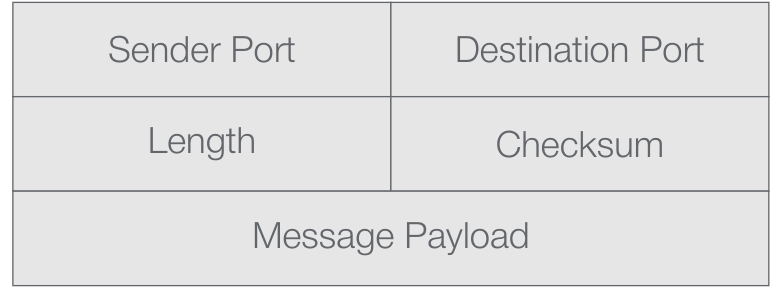
\includegraphics[width=0.5\linewidth]{Images/livello_trasporto/UDP_header.png}
    \caption{Segmento UDP.}
\end{figure}

In particolare:
\begin{itemize}
    \item \textbf{Numero di porta sorgente} (16 bit). 
    \item \textbf{Numero di porta di destinazione} (16 bit).
    \item \textbf{Lunghezza} (16 bit): header + data, dove l'header è sempre 8 byte.
    \item \textbf{Checksum} (16 bit).
\end{itemize}

\subsection{Campo Checksum}
Questo campo è stato aggiungo perchè non tutte le connessioni a livello H2N hanno un controllo dell'errore e inoltre, il controllo dell'errore con checksum a livello IP controlla solo il datagram IP.
Quindi, a livello di trasporto, non ci sarebbe stato nessun modo di avere un ripristino dall'errore.
\\
Nel pratico:
\begin{itemize}
    \item \textbf{Sorgente:} tratta il contenuto del segmento come una sequenza di numeri interi a 16 bit, somma il contenuto dei segmenti in complemento a uno e invia il valore del checksum nel campo del segmento UDP.
    \item \textbf{Desrinatario:} calcola il checksum del segmento ricevuto e verifica se il valore del checksum calcolato è uguale a quello ricevuto.
\end{itemize}

\vspace*{0.02\textheight}
\textbf{ESEMPIO:}
\vspace*{0.01\textheight}
\begin{center}
    \begin{tabular}{ c | c }
        \hline
        \textbf{Word 1} & 0110011001100110 \\
        \textbf{Word 2} & 0101010101010101 \\
        \textbf{Word 3} & 0000111100001111 \\
        \hline
        \textbf{Somma} & 1100101011001010 \\
        \hline
        \textbf{Complemento a 1} & 0011010100110101 \\
        \hline
    \end{tabular}
\end{center}
Il destinatario calcola il proprio checksum del segmento UDP, senza calcolare il complemento a uno:
\begin{itemize}
    \item \textbf{OK:} checksum destinazione + checksum UDP = 1111111111111111.
    \item \textbf{ERRORE:} Checksum destinazione + checksum UDP != 1111111111111111.
\end{itemize}

\section{Protocollo TCP}
Il protocollo TCP fornisce un livello di trasporto affidabile e orientato alla connessione. Ha alcuni servizi aggiuntivi rispetto a UDP:
\begin{itemize}
    \item \textbf{Orientato alla connessione:} include le fasi di  stabilimento, utilizzo e chiusura della connessione.
    \item \textbf{Orientato al flusso di dati:} considera il flusso di dati dall'host mittente al destinatario.
    \item \textbf{Trasferimento con buffer:} i dati vengono memorizzati in un buffer e quindi inseriti in un pacchetto quando il buffer è pieno.
    \item \textbf{Connessione full-duplex (bidirezionale):} una volta stabilita la connessione, è possibile il trasferimento simultaneo in entrambe le direzioni della connessione.
\end{itemize}

\subsection{Affidabilità}
Affidabile significa che TCP gestisce il trasferimento di un flusso di dati con la sequenza corretta (ACK + timeout + ritrasmissione):
\begin{itemize}
    \item Ogni trasmissione riuscita viene notificata (\textbf{ACK}) dall'host ricevente.
    \item Se l'host mittente non riceve una conferma entro un intervallo di tempo predefinito (\textbf{timeout}), il mittente ritrasmette i dati.
    \item Gli \textbf{ACK} e le \textbf{ritrasmissioni} dovute a eventuali perdite vengono gestite in modo trasparente rispetto al processo applicativo.
\end{itemize}

\subsection{Trasferimento con buffer}
Per risolvere molti dei problemi evidenziati sopra, il livello TCP deve necessariamente utilizzare un buffer per evitare:
\begin{itemize}
    \item Invio asincrono dei dati rispetto al processo applicativo.
    \item Tempi di trasmissione differenti.
    \item Capacità di invio e ricezione differenti.
    \item Segmenti persi o fuori sequenza.
\end{itemize}
Inoltre, il protocollo TCP ha altri due compiti fondamentali:
\begin{enumerate}
    \item \textbf{Controllo della congestione:} l'host mittente deve ridurre la velocità di trasmissione dei pacchetti quando la rete è congestionata.
    \item \textbf{Controllo del flusso:} l'host mittente non deve sovraccaricare l'host ricevente.
\end{enumerate}

\begin{figure}[!htb]
    \centering
    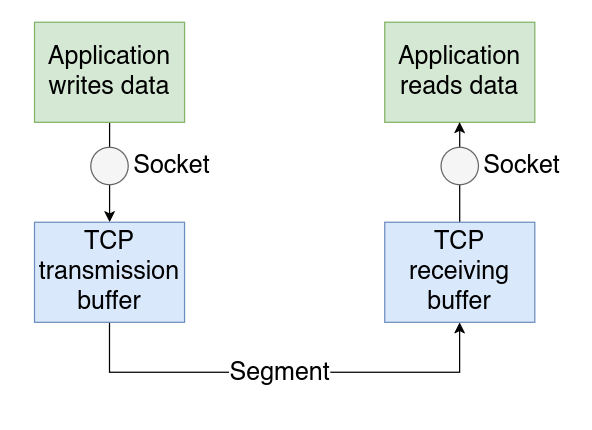
\includegraphics[width=0.5\linewidth]{Images/livello_trasporto/TCP_buffer.png}
    \caption{Esempio di utilizzo del buffer TCP.}
\end{figure}

Un'applicazione può anche indicare a TCP di inviare i dati presenti nel buffer, senza attendere che quest'ultimo sia pieno.

\section{TCP Segment}
L'insieme di dati che il livello TCP richiede di trasferire al livello IP è chiamato segmento TCP ed è formato da una parte di header e da una parte di byte di dati.

\begin{figure}[!htb]
    \centering
    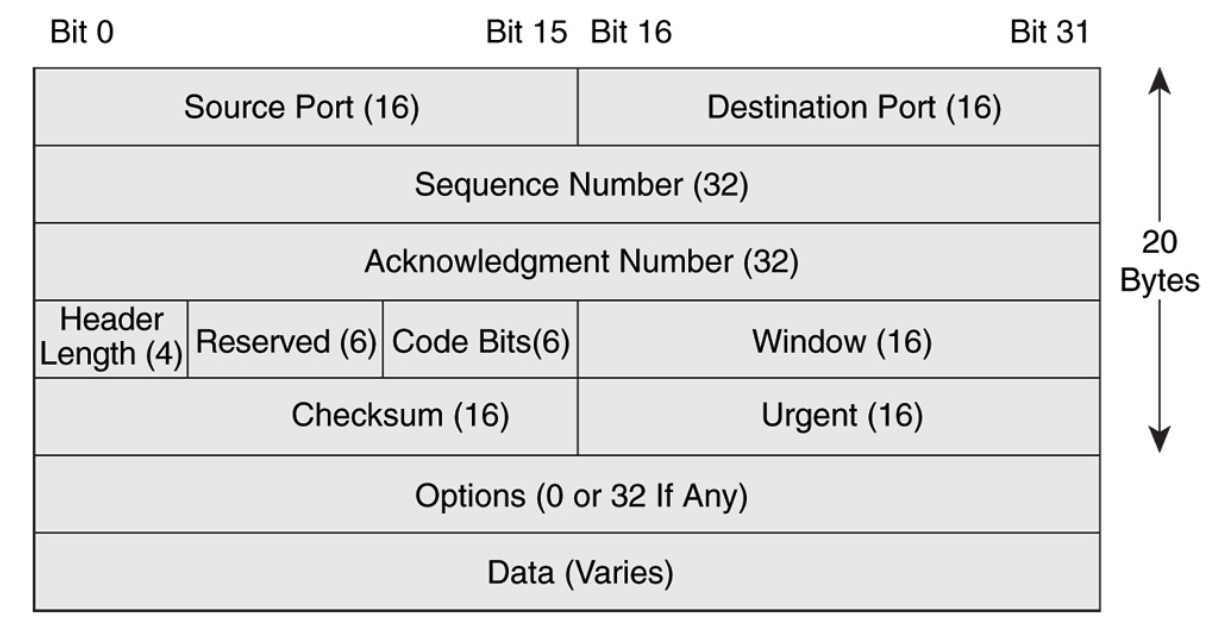
\includegraphics[width=0.7\linewidth]{Images/livello_trasporto/TCP_segment.png}
    \caption{Esempio di utilizzo del buffer TCP.}
\end{figure}

Nello specifico:
\begin{itemize}
    \item \textbf{Porta sorgente} (16 bit).
    \item \textbf{Porta di destinazione} (16 bit).
    \item \textbf{Sequence number} (32 bit): sequence number relativo al flusso di byte trasmesso.
    \item \textbf{Acknowledgment number} (32 bit): ACK relativo al sequence number del flusso di byte ricevuto.
    \item \textbf{Lunghezza dell'header} (4 bit): lunghezze in multipli di 32 bit dell'header, se non ha opzioni è sempre 20 byte.
    \item \textbf{Reserved} (6 bit): riservato per usi futuri.
    \item \textbf{Code bit} (6 bit): usato per le varie flag:
    \begin{itemize}
        \item URG: dati segnati come urgenti dal layer applicativo.
        \item ACK: valore dell'ACK è valido.
        \item PSH: i dati devono essere passati all'applicazione subito.
        \item SYN, FIN, RST: usati per stabilire, chiudere o interropere una connessione.
    \end{itemize}
    \item \textbf{Dimensione della finestra} (16 bit): indica il numero di byte che il destinatario è disposto ad accettare.
    \item \textbf{Checksum} (16 bit): controllo dell'integrità come nell'UDP.
    \item \textbf{Urgent} (16 bit): puntatore alla fine dei dati urgenti.
    \item \textbf{Opzioni} (0-32 bit): campi opzionali di varie dimensioni (come MSS - maximun segment size).
    \item \textbf{Padding di zeri} se necessario.
\end{itemize}
Alcuni esempi di dati urgenti posso essere i segnali come \textit{Ctrl + Z} o \textit{Ctrl + C}, in modo che possano arrivare immediatamente. Quando vengono ricevuti, saltano direttamente lo stream di byte e arrivano all'applicazione. Sono posizionati all'inzio del segmento, per questo il puntatore Urgent punta alla loro fine.

\newpage
\section{Inizializzare e chiudere una connessione TCP}
Nel protocollo TCP, il mittente e il destinatario stabiliscono la connessione e inizializzano le variabili dei segmenti prima di iniziare il trasferimento, utilizzando un modello \textbf{client/server}. \\
Per stabilire una connessione il client invia un segmento particolare, dove imposta il campo \textbf{SYN} a 1, al server. Deve contenere:
\begin{itemize}
    \item La porta del server.
    \item L'\textbf{ISN (Initial Sequence Number)} del client, un numero a 32 bit pseudo randomico, da cui inizierà la numerazione.
    \item L'\textbf{MRW (Maximum Receive Window)}, ossia il numero di byte che il client può ricevere nel buffer.
    \item L'\textbf{MSS (Maximum Segment Size)}, la grandezza massima del segmento, anche se non sempre è inviata.
\end{itemize}
Questo segmento TCP non contiene nessun dato, ma solo l'header.
Il server, al sua volta, risponderà con un segmento con \textbf{SYN} a 1 e con gli stessi campi, ma con i valori riferiti a lui e con un ACK con valore dell'\textbf{ISN} del client aumentato di uno. Infine, il client risponderà con un \textbf{ACK} del valore dell'\textbf{ISN} del server aumentato di uno.

\begin{figure}[!htb]
    \centering
    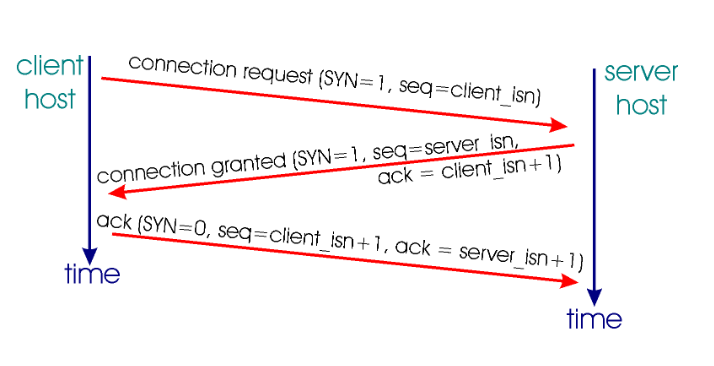
\includegraphics[width=0.7\linewidth]{Images/livello_trasporto/Three-way-hand.png}
    \caption{Esempio di three-way-handshaking.}
\end{figure}

Per chiudere una connessione in modo pulito, il client deve mandare un segmento con il campo \textbf{FIN} a 1 al server, il quale dopo aver risposto al client con un \textbf{ACK}, chiude la connessione lato client e invia a sua volta un segmento con campo \textbf{FIN} a 1 al client. Infine, il client dopo aver ricevuto il \textbf{FIN} del server gli invia un \textbf{ACK}. Il server appena riceve l'\textbf{ACK} chiude la connessione, il client la chiude dopo un tempo di timeout. \\
Un altro modo per interropere una connessione è impostare il campo \textbf{RST} a 1, questo farà si che l'altro nodo chiuda immediatamente la connessione e che tutte le risorse vengano liberate.

\begin{figure}
    \begin{minipage}{.45\linewidth}
        \centering
        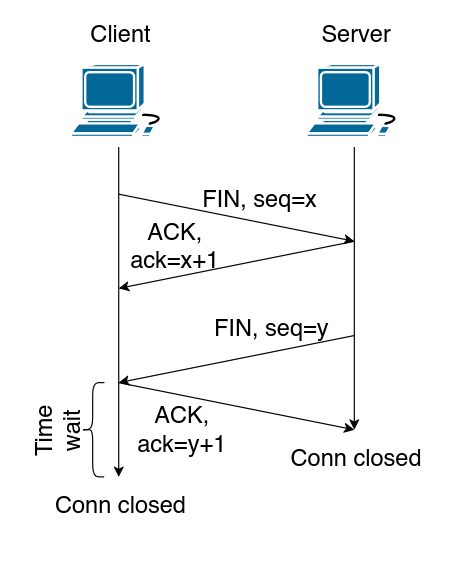
\includegraphics[width=0.6\linewidth]{Images/livello_trasporto/FIN.png}
        \caption{Chiusura pulita di una connessione.}
    \end{minipage}
    \begin{minipage}{.45\linewidth}
        \centering
        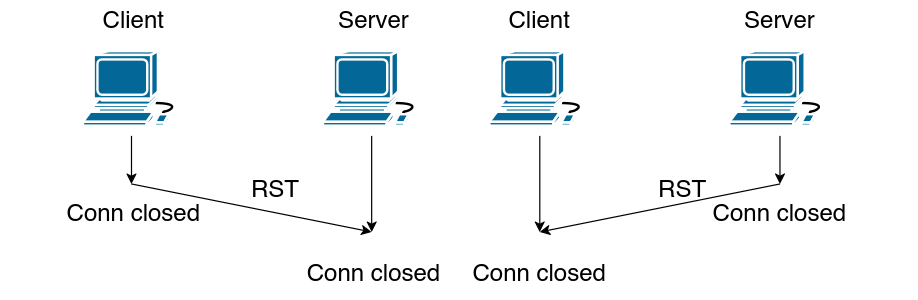
\includegraphics[width=1.2\linewidth]{Images/livello_trasporto/RST.png}
        \caption{Interruzione di una connessione.}
    \end{minipage}
\end{figure}

\section{Affidabilotà nel protocollo TCP}
Ci sono diversi meccanismi per garantire affidabilità in modo trasparente rispetto al processo applicativo:
\begin{itemize}
    \item \textbf{ACK.}
    \item \textbf{Timeout.}
    \item \textbf{Ritrasmissione.}
\end{itemize}
Ogni trasmissione riuscita viene \textbf{confermata} dall'host ricevente.Se l'host mittente non riceve una conferma entro il \textbf{timeout}, il mittente ritrasmette i \textbf{dati}.

\subsection{Stima del Timeout}
La stima del timeout viene fatto usando l'\textbf{RTT (Round Trip Time)}. Il valore è molto importante calcolarlo bene, perchè se troppo basso si rischia di dover inviare il segmento più volte, se troppo alto, invece, si ha una lenta risposta ai segmenti persi. In generale, il timeout deve essere dell'RTT.
Ci sono due modi per misusare il Round Trip Time:
\begin{enumerate}
    \item \textbf{SamlpleRTT:} misura il tempo dall'invio del segmento alla ricezione dell'ACK, varia più volte dinamicamente.
    \item \textbf{EstimatedRTT:} media pesata per sapere l'RTT a un tempo \textbf{t}: 
    \[
        \text{EstimatedRTT}(t) = (1 - \alpha) \cdot \text{EstimatedRTT}(t-1) + \alpha \cdot \text{SampleRTT}(t)
    \]
    Dove, dato un numero $n$ di casi:
    \[
        \alpha = \frac{1}{n+1}
    \]
\end{enumerate}
Attualmente, il \textbf{timeout} è calcolato usando l'EstimatedRTT e un piccolo margine:
\[
    \text{Timeout}(t) = \text{EstimatedRTT}(t) + Dev(t)
\]
Dove:
\[
    Dev(t) = (1-\alpha)Dev(t-1) \space + \space \alpha \cdot |\text{SampleRTT}(t)-\text{EstimatedRTT(t)}|
\]

\newpage
\section{Gestione del Buffer TCP}
TCP, essendo parte del Sistema Operativo e non del layer applicativo, deve riuscire a gestire tutte gli eventi asincroni che accadono. Infatti, il protocollo TCP non sa quando un processo vorrà inviare i dati o quando li vorrà ricevere. Per questo si inseriscono temporaneamente i dati dentro un \textbf{buffer}.

\begin{boxDef}
\textbf{\textcolor{brown}{Alcune definizioni:}}
\begin{itemize}
    \item \textbf{RTT:} tempo di un segmento per arrivare a destinazione e tornare indietro.
    \item \textbf{Tempo di propagazione ($\text{T}_p$):} $\frac{\text{RTT}}{2}$.
    \item \textbf{Utilizzo (U):} percentuale di utilizzo delle risorse.
    \item \textbf{Frequenza di Trasmissione ($\text{T}_r$).} 
    \item \textbf{Packet Lenght:} $L(pkt)$.
    \item \textbf{Tempo di trasmissione di un pacchetto (TT):} $\frac{L(pkt)}{\text{T}_r}$.
    \item \textbf{Tempo di trasferimento di un segmento(T):} T = $[\frac{\text{RTT}}{2} + L(pkt)] + \frac{\text{RTT}}{2}$
\end{itemize}
\end{boxDef}
I buffer servono per passare da un meccanismo \textbf{Stop-and-Wait} a uno in \textbf{pipeline}. Devono essere implementati sia dal lato del mandante che del destinatario, insieme a protoccoli \textbf{Sliding Windows} per sapere quanti pacchetti mandare senza ricevere il loro ACK.

\begin{figure}[!htb]
    \centering
    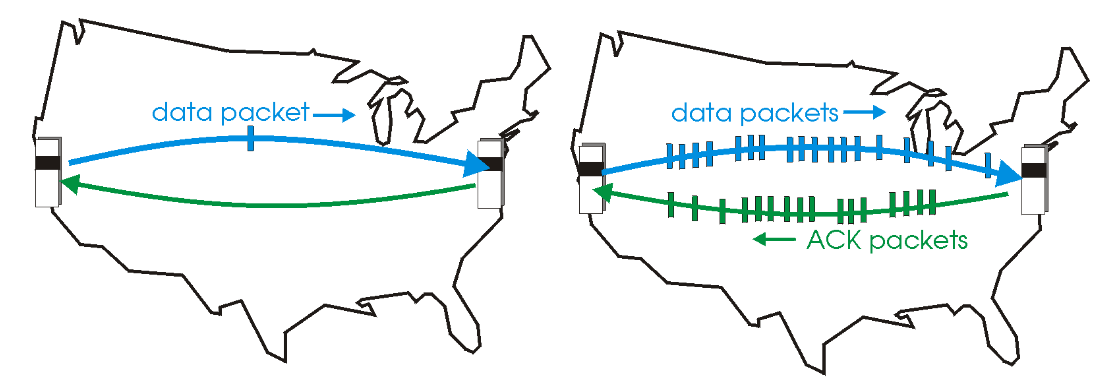
\includegraphics[width=0.8\linewidth]{Images/livello_trasporto/Stop-and-Wait.png}
    \caption{Protocolli Stop-and-Wait e con Pipeline.}
\end{figure}

\begin{figure}[!htb]
    \centering
    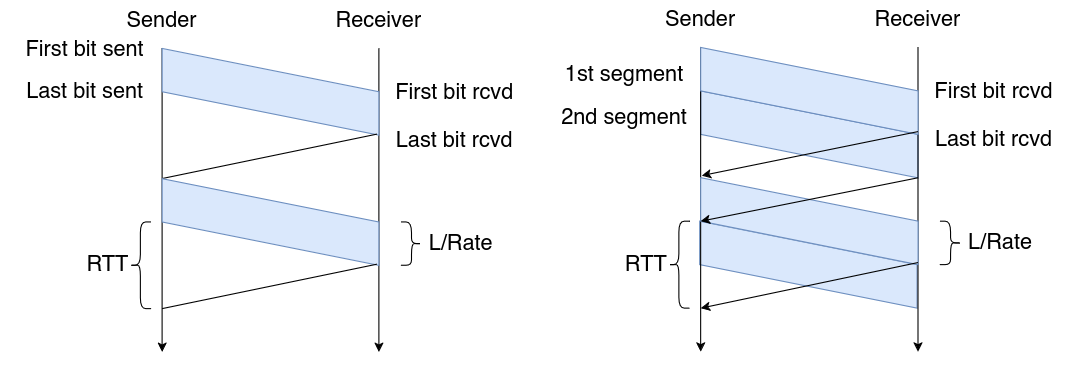
\includegraphics[width=0.8\linewidth]{Images/livello_trasporto/Pipeline.png}
    \caption{Protocolli Stop-and-Wait e con Pipeline.}
\end{figure}

\newpage
\subsection{Sliding Windows}
Il mittente assegna a ciascun segmento un numero di sequenza \textbf{segment\_no} nelll'intervallo $[0, 2^{32} - 1]$.
\begin{center}
    \begin{minipage}{.45\linewidth}
        \begin{boxDef}
        \textbf{\textcolor{brown}{Mandante}} \\
        In ogni momento, il mittente mantiene una sliding window sugli indici di segmento e solo quelli all'interno della finestra possono essere trasmessi. La dimensione della finestra utile del mittente è controllata dal destinatario. Usa tre variabili:
            \begin{itemize}
                \item \textbf{Sender Window Size (SWS):} il massimo di segmenti che può mandare senza ricevere un ACK.
                \item \textbf{Last ACK Received (LAR):} numero di sequenza dell'ultimo ACK ricevuto.
                \item \textbf{Last Segment Send (LSS):} numero di sequenza dell'ultimo segmento inviato.
            \end{itemize}
        \textbf{NB:} \[\text{LAS} - \text{LSR} \ge \text{RWS}\]
        \end{boxDef}
    \end{minipage}
    \begin{minipage}{.45\linewidth}
        \begin{boxDef}
        \textbf{\textcolor{brown}{Ricevente}} \\
        In qualsiasi momento, il destinatario mantiene una sliding window sugli indici dei segmenti ricevuti. La dimensione della finestra e le modalità di gestione dipendono dall'algoritmo utilizzato. Usa tre variabili:
            \begin{itemize}
                \item \textbf{Receive Window Size (RWS):} indica il numero massimo di segmenti fuori sequenza che può accettare.
                \item \textbf{Largest Accetable Segment (LAS):} numero di sequenza più grande che può accettare. 
                \item \textbf{Last Segment Received (LSR):} numero di sequenza dell'ultimo segmentoricevuto in ordine.
            \end{itemize}
        \textbf{NB:} \[\text{LSS} - \text{LAR} \ge \text{SWS} \]
        \end{boxDef}
    \end{minipage}
\end{center}

\begin{figure}[!htb]
    \begin{minipage}{.47\linewidth}
        \centering
        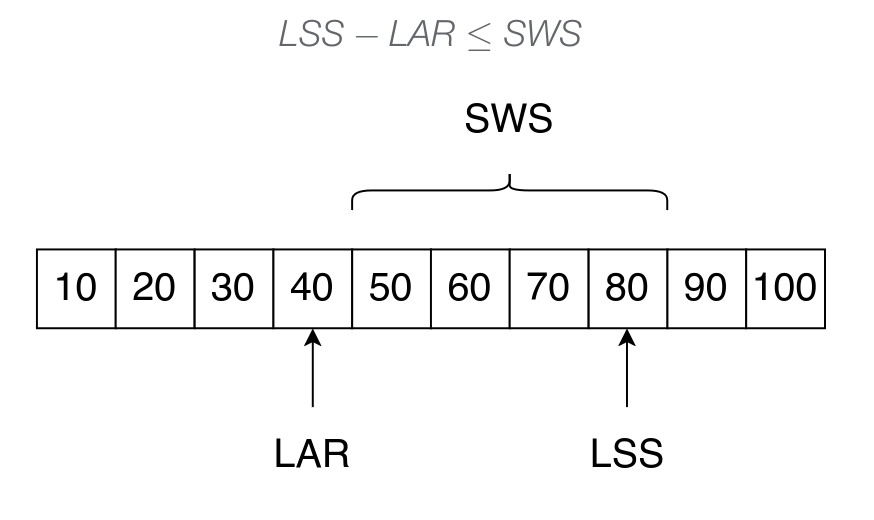
\includegraphics[width=0.8\linewidth]{Images/livello_trasporto/Mandante.png}
        \caption{Chiusura pulita di una connessione.}
    \end{minipage}
    \begin{minipage}{.47\linewidth}
        \centering
        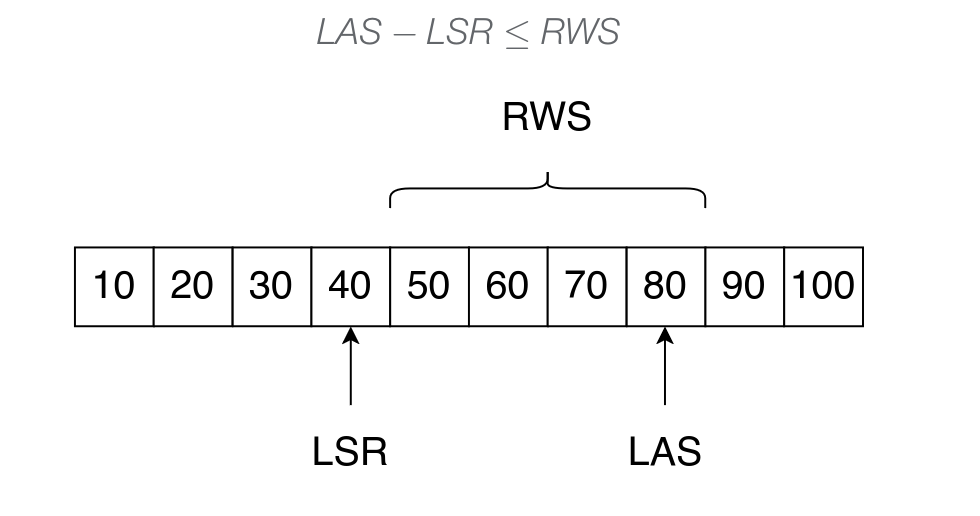
\includegraphics[width=0.9\linewidth]{Images/livello_trasporto/Ricevente.png}
        \caption{Interruzione di una connessione.}
    \end{minipage}
\end{figure}

\subsection{Flow Control}
L'obiettivo è non far inviare al mandante più dati di quelli che il buffer del destinatario può contenere. Il ricevitore comunica esplicitamente al mittente la quantità di spazio libero nel buffer di ricezione TCP e varia dinamicamente, quindi ogni segmento ACK comunica al mittente il numero massimo di byte ricevibili.

\begin{figure}[!htb]
    \centering
    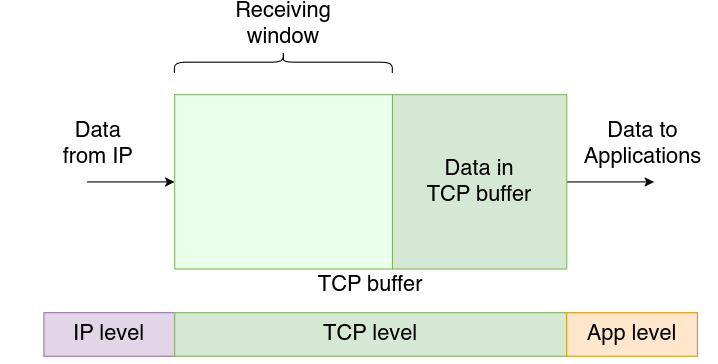
\includegraphics[width=0.6\linewidth]{Images/livello_trasporto/FlowControl.png}
    \caption{Buffer TCP.}
\end{figure}

L'ACK contiene due informazioni:
\begin{enumerate}
    \item Quanti byte ha ricevuto il recipiente.
    \item Quanti byte può ancora ricevere in quel momento.
\end{enumerate}

\[
\textbf{Advertised Window} = \text{MaxRcvBuffer} -((\text{NextByteExpected} - 1) - \text{LastByteRead})
\]

\[
\textbf{EffectiveWindow} = \text{AdvertisedWindow} - (\text{LastByteSent} - \text{LastByteAcked})
\]

Quando il mandante riceve $\textbf{Advertised Window} = 0$, teoricamente non può più mandare dati e per questo non riesce a capire quando può ricominciare a mandare dati. La soluzione nel protocollo TCP è mandare costantemente mandare un segmento con un byte di dato.

\subsection{Congestion Control}
La congestione in una rete può causare diversi problemi, come la perdita di pacchetti oppure tempi di delay molto elevati.
Ci sono due modi per approcciarsi alla gestione della congestione:
\begin{enumerate}
    \item \textbf{Controllo end-to-end:} approccio usato dal protocollo TCP, non viene gestito dalla rete, ma si guardano i pacchetti persi e il tempo di delay.
    \item \textbf{Controllo di rete:} i router dicono ai nodi terminali lo stato della congestione della rete.
\end{enumerate}

\begin{figure}[!htb]
    \centering
    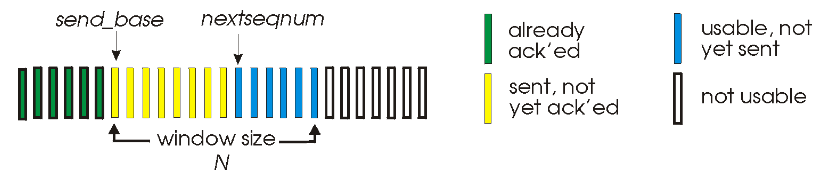
\includegraphics[width=0.8\linewidth]{Images/livello_trasporto/WindowSize.png}
    \caption{Dimensione della finestra nel TCP.}
\end{figure}

Le prestazioni nel protocollo TCP vengono misurate tramite il \textbf{Throughput}:
\[
\textbf{Throughput} = \frac{w \space\cdot MSS}{RTT}
\]
Dove $w$ è il numero di segmenti della finestra.
Esistono diversi algortimi per evitare la congestione della rete:

\subsubsection{Slow Start}
Inizia con la dimensione della finestra di congestione pari a 1 e poi in modo esponenziale aumenta fino al threshold.

\begin{bashbox}
ffor each ACK segment do
    CW++
    if timeout OR CW > threshold then
        break
\end{bashbox}


\subsubsection{Tahoe Algorithm}
Cresce in modo esponenziale fino al threshold, poi incrementa di 1.

\textbf{\{Slow start ended, CW $\ge$ threshold\}}
\begin{bashbox}
iif not loss then
    for all ACK segment
        CW++
else
    threshold = CW/2
    CW = 1
    do slow start
\end{bashbox}


\subsubsection{Reno Algorithm}
Controlla due tipi di errore:
\begin{enumerate}
    \item \textbf{Timeout:} riduce la finestra di congestione a 1.
    \item \textbf{Tre ACK duplicati:} riduce la finestra di metà.
\end{enumerate}

\textbf{\{Slow start ended, CW $\ge$ threshold\}}
\begin{bashbox}
iif not loss then
    for all ACK segment 
        CW++
else
    threshold = CW/2
    if Loss detected by timeout then
        CW = 1
        do slow start
    if loss detected by triple ACK then
        CW = CW/2
\end{bashbox}
Reno, in confronto a Tohoe, ha una recupero molto più veloce, ma ormai, entrambi sono obsoleti.

\subsubsection{Vegas Algorithm}
Il timeout è basato sull'RTT e ha un contatore che controlla ogni pacchetto.

\begin{bashbox}
xx(t) = [WSize(t) - WSize(t-1)] / [RTT(t) - RTT(t-1]
if x(t) > 0
    CW = CW - CW/8
else
    CW = CW + MSS
\end{bashbox}
Se aumenta la congestione aumenta pure l'RTT e viceversa. La finestra di congestione cambia ogni $2 \cdot \text{RTT}$.

\subsubsection{BIC (Binary Increase Congestion)}
Mantiene 4 valori diversi di finestre di congestione:
\begin{enumerate}
    \item \textbf{Attuale.}
    \item \textbf{Massima.}
    \item \textbf{Minima.}
    \item \textbf{Prevista (valore fra massimo e minimo).}
\end{enumerate}
Nello specifico: 
\begin{enumerate}
    \item Quando la differenza tra la finestra minima e quella massima è ampia, si ricorre a una crescita aggressiva della finestra (\textbf{incremento additivo}).
    \item Quando la finestra corrente raggiunge quella prevista senza errori, la finestra minima diventa quella prevista.
    \item In caso di errore, la finestra massima assume il valore della finestra corrente. La finestra corrente si riduce al nuovo valore minimo.
    \item Man mano che le finestre minime e massime si restringono, la ricerca diventa meno aggressiva.
\end{enumerate}

\subsubsection{CUBIC}
Evoluzione di BIC, mantiene la sua stabilità e scalabilità, ma aumenta la fairness. Infatti, la dimensione della finestra di congestione dipende la tempo e non dall'RTT.

\subsection{Buffer Bloating}
Problema regolato dalla presenza di buffer molto grandi nella rete, tipicamente di dimensioni variabili. Si verifica in presenza di trasferimenti di dati di lunga durata e dalla presenza di più flussi TCP simultanei. Quando i buffer sono pieni, l'RTT è così elevato che il timeout per la perdita di pacchetti rallenta l'intervento del controllo della congestione. Il risultato è il calo del throughput a causa dei ritardi e un elevato tasso di perdita di pacchetti.
Esistono alcune proposte per risolvere questo problema come:
\begin{itemize}
    \item \textbf{CoDel Algortihm (Controlled Delay)} come algoritmo di AQM (Adaptive Queue Management) per gestire la grandezza dei buffer in modo dinamico per più flussi TCP.
    \item \textbf{Google SPDY.}
    \item \textbf{HTTP/2.}
\end{itemize}

\chapter{Socket Programming}
\section{API (Application Program Interface)}
\begin{boxDef}
\textbf{\textcolor{brown}{API:}} meccanismo utilizzato come ponte tra il sistema operativo e l'applicazione di rete che può essere utilizzato per sviluppare applicazioni. Fa parte del sistema operativo e consente ai processi applicativi di utilizzare protocolli di rete, definendo:
\begin{itemize}
    \item Le operazioni consentite.
    \item Gli argomenti per ciascuna operazione.
\end{itemize}
\end{boxDef}
L'\textbf{API} per \textbf{Socket}, inizialmente definita per \textbf{BSD Unix} per utilizzare i protocolli \textbf{ TCP/IP}, è disponibile su vari sistemi operativi.

\subsection{Socket}
\begin{boxDef}
\textbf{\textcolor{brown}{Socket:}} sono \textbf{API} che consentono ai programmatori di gestire le comunicazioni tra \textbf{processi}. Consentono la comunicazione tra processi che possono risiedere su \textbf{host} diversi e costituiscono quindi lo strumento di base per la creazione di servizi di rete.
In pratica, permettono a un programmatore di effettuare trasmissioni \textbf{TCP} e \textbf{UDP} senza doversi preoccupare dei dettagli di livello inferiore, che sono gli stessi per ogni comunicazione.
Forniscono inoltre un'interfaccia diretta al livello di rete, le \textbf{socket raw}. Vengono utilizzati in un ambiente \textbf{Linux/Unix} in modo simile ai file per le operazioni di \textbf{I/O}.
\end{boxDef}
Forniscono una serie di funzioni:
\begin{itemize}
    \item \textbf{socket():} crea un punto di comunicazione.
    \item \textbf{bind():} fissa un indirizzo locale alla socket.
    \item \textbf{liste():} si mette a disposizione per accettare richieste.
    \item \textbf{accept():} aspetta una richiesta di connessione.
    \item \textbf{write():} manda i dati tramite la connessione.
    \item \textbf{read():} receve i dati dalla connessione.
    \item \textbf{close():} chiude la connessione.
\end{itemize}

\section{Creare e gestire una connessione}
Inizialmente, va dichiarato al sistema operativo dell'intenzione di stabilire una \textbf{connessione} con specifica delle caratteristiche. Successivamente, si possono aprire le connessioni (diverse tra lato \textbf{server} e lato \textbf{client}):
\begin{itemize}
    \item Il server presume di definire la connessione prima del client e attende che il client si connetta alla porta specificata.
    \item Il client presume che il server sia già attivo e tenta di connettersi specificando l'indirizzo e la porta del server.
\end{itemize}
Lo scambio di dati è \textbf{bidirezionale} (trasmissione e ricezione). Alla fine della comunicazione, la connessione viene chiusa.\\

\vspace*{0.02\textheight}
\textbf{Creazione del socket:}
\begin{cbox}
ddescriptor = socket(protofamily, type, protocol)
\end{cbox}
Dove:
\begin{itemize}
    \item \textbf{Descriptor:} handler del socket, int.
    \item \textbf{Protocol Family:} specifica il dominio di comunicazione:
    \begin{itemize}
        \item \textbf{AF\_INET:} protocolli Internet IPv4.
        \item \textbf{AF\_INET6:} protocolli Internet IPv6.
        \item \textbf{AF\_UNIX:} comunicazioni locali (stessa macchina).
        \item \textbf{AF\_PACKET:} accesso diretto al livello di collegamento.
    \end{itemize}
    \item \textbf{Socket Type:} specifica la semantica della comunicazione:
    \begin{itemize}
        \item \textbf{SOCK\_STREAM:} connessione TCP.
        \item \textbf{SOCK\_DGRAM:} connessione UDP.
        \item \textbf{SOCK\_RAW:} accesso grezzo al protocollo. 
    \end{itemize}
\end{itemize}
Non tutte e le combinazioni sono valide.

\vspace*{0.02\textheight}
\textbf{Binding del socket:}
\begin{cbox}
bbind(socket, localaddr, addrlen)
\end{cbox}
Dove:
\begin{itemize}
    \item \textbf{Socket:} descriptor del socket.
    \item \textbf{Local Address:} indirizzo su cui mettersi in ascolto.
    \item \textbf{Address Len:} lunghezza dell'indirizzo.
\end{itemize}

\vspace*{0.02\textheight}
\textbf{Mettersi in ascolto sul socket:}
\begin{cbox}
llisten(socket, queuesize)
\end{cbox}
Dove:
\begin{itemize}
    \item \textbf{Socket:} descriptor del socket.
    \item \textbf{Queue Size:} numero di richieste in sospeso consentite.
\end{itemize}

\vspace*{0.02\textheight}
\textbf{Accettare nuove connessioni:}
\begin{cbox}
nnewsock = accept(socket, caddress, caddresslen)
\end{cbox}
Dove:
\begin{itemize}
    \item \textbf{Socket:} descriptor del socket.
    \item \textbf{Client address:} puntatore all'indirizzo del client.
    \item \textbf{Dimensione dell'indirizzo:} puntatore a un intero con la dimensione dell'indirizzo del client.
    \item \textbf{New Socket:} descriptor del nuovo socker creato.
\end{itemize}

\vspace*{0.02\textheight}
\textbf{Creare una nuova connessione:}
\begin{cbox}
cconnect(socket, saddress, saddresslen)
\end{cbox}
Dove:
\begin{itemize}
    \item \textbf{Socket:} descriptor del socket.
    \item \textbf{Server address:} puntatore all'indirizzo del client.
    \item \textbf{Dimensione dell'indirizzo:} puntatore a un intero con la dimensione dell'indirizzo del client.
\end{itemize}

\vspace*{0.02\textheight}
\textbf{Inviare dati:}
\begin{cbox}
ssend(socket, data, length, flags)
\end{cbox}
Dove:
\begin{itemize}
    \item \textbf{Socket:} descriptor del socket.
    \item \textbf{Data:} puntatore ai dati da inviare.
    \item \textbf{Dimensione dei dati:} pintero con la dimensione dei dati.
    \item \textbf{Flags:} flag da specificare nel caso.
\end{itemize}

\begin{figure}[!htb]
    \centering
    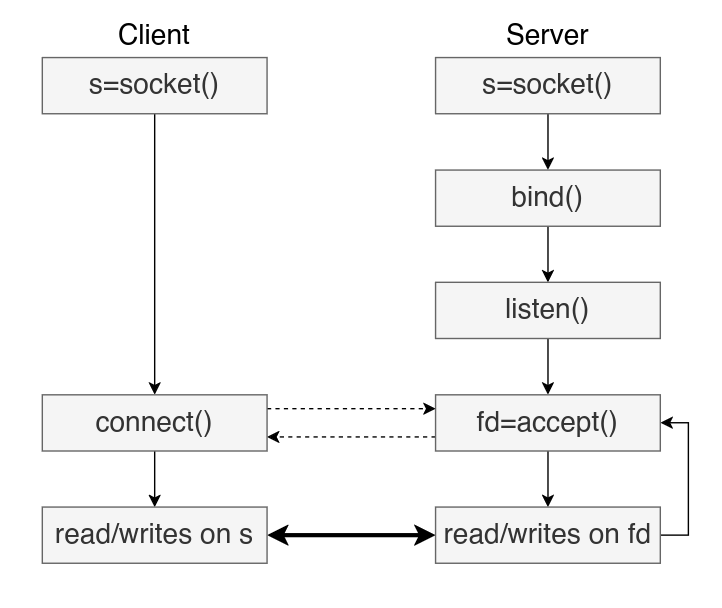
\includegraphics[width=0.5\linewidth]{Images/Socket_Programming/Socket.png}
    \caption{Connessione e comunicazione con socket.}
\end{figure}

Per le connessioni UDP, a differenza delle connessioni TCP, non c'è bisogno di mettersi in ascolto. Si possono mandare dati e ricevere dati direttamente sulla rete, usando:

\begin{cbox}
rrecvfrom(sockfd, *buf, size, flags, *src_addr, *addrlen)
sendto(sockfd, *buf, size, flags, *dst_addr, addrlen)
\end{cbox}
Queste funzioni sostituiscono le syscall write() e read().

\subsection{Codice C Server Side:}
\begin{cbox}
/* A simple server using TCP
The port number is passed as an argument */

#include <stdio.h>
#include <stdlib.h>
#include <unistd.h>
#include <string.h>
#include <sys/types.h>
#include <sys/socket.h>
#include <netinet/in.h>

void error(char *msg){
    perror(msg);
    exit(1);
}

int main(int argc, char *argv[]){
    int sockfd, newsockfd, portno, clilen;
    char buffer[256];
    struct sockaddr_in serv_addr, cli_addr;
    int n;
    
    if (argc < 2) {
        fprintf(stderr,"ERROR, no port provided\n");
        exit(1);
    }
    
    sockfd = socket(AF_INET, SOCK_STREAM, 0);
    if (sockfd < 0)
        error("ERROR opening socket");
        
    bzero((char *) &serv_addr, sizeof(serv_addr));
    portno = atoi(argv[1]);
    serv_addr.sin_family = AF_INET;
    serv_addr.sin_addr.s_addr = INADDR_ANY;
    serv_addr.sin_port = htons(portno);
    
    if (bind(sockfd, (struct sockaddr *) &serv_addr, sizeof(serv_addr)) < 0)
        error("ERROR on binding");
    
    listen(sockfd, 5);
    clilen = sizeof(cli_addr);
    newsockfd = accept(sockfd, (struct sockaddr *) &cli_addr, &clilen);
    if (newsockfd < 0) 
        error("ERROR on accept");
    
    bzero(buffer, 256);
    n = read(newsockfd, buffer, 255);
    if (n < 0)
        error("ERROR reading from socket");
        
    printf("Here is the message: %s\n",buffer);
    n = write(newsockfd, "I got your message",18);
    if (n < 0)
        error("ERROR writing to socket");
    
    return 0;
}
\end{cbox}

\subsection{Codice C Client Side:}
\begin{cbox}
#include <stdio.h>
#include <unistd.h>
#include <stdlib.h>
#include <string.h>
#include <sys/types.h>
#include <sys/socket.h>
#include <netinet/in.h>
#include <netdb.h>

void error(char *msg){
    perror(msg);
    exit(0);
}

int main(int argc, char *argv[]){
    int sockfd, portno, n;
    struct sockaddr_in serv_addr;
    struct hostent *server;
    char buffer[256];
    
    if (argc < 3) {
        fprintf(stderr,"usage %s hostname port\n", argv[0]);
        exit(0);
    }
    
    portno = atoi(argv[2]);
    sockfd = socket(AF_INET, SOCK_STREAM, 0);
    if (sockfd < 0)
        error("ERROR opening socket");

    server = gethostbyname(argv[1]);
    if (server == NULL) {
        fprintf(stderr,"ERROR, no such host\n");
        exit(0);
    }
    
    bzero((char *) &serv_addr, sizeof(serv_addr));
    serv_addr.sin_family = AF_INET;
    bcopy((char *)server->h_addr, (char *)&serv_addr.sin_addr.s_addr, server->h_length);
    serv_addr.sin_port = htons(portno);

    if (connect(sockfd, (const struct sockaddr *) &serv_addr, sizeof(serv_addr) < 0)
        error("ERROR connecting");
    
    printf("Please enter the message: ");
    bzero(buffer, 256);
    fgets(buffer, 255, stdin);
    n = write(sockfd, buffer, strlen(buffer));
    if (n < 0)
        error("ERROR writing to socket");
    
    bzero(buffer, 256);
    n = read(sockfd, buffer, 255);
    if (n < 0)
        error("ERROR reading from socket");
    printf("%s\n", buffer);
    
    return 0;
}
\end{cbox}

\subsection{Codice Python Server Side:}
\begin{pybox}
#!/usr/bin/env python3
import socket
import sys
import time

HOST = '127.0.0.1' # Standard loopback interface address (localhost)
PORT = int(sys.argv[1]) # Port to listen on

with socket.socket(socket.AF_INET, socket.SOCK_STREAM) as s:
    s.bind((HOST, PORT))
    s.listen()
    conn, addr = s.accept()
    #print('Connected by', addr)
    data = conn.recv(1024)
    print('Here is the message: %s'% data.decode('utf-8'))
    conn.sendall('I got your message'.encode('utf-8'))
    # socket must be closed by client! sleep for 1 second
    time.sleep(1) # otherwise socket goes to TIME_WAIT!
\end{pybox}

\subsection{Codice Python Client Side:}
\begin{pybox}
#!/usr/bin/env python3
import socket
import sys
HOST=sys.argv[1]
PORT=int(sys.argv[2])
with socket.socket(socket.AF_INET, socket.SOCK_STREAM) as s:
    s.connect((HOST, PORT))
    msg = input('Please enter the message: ')
    s.sendall(msg.encode('utf-8'))
    data = s.recv(1024)
    s.close()
    print('Received: %s'% data.decode('utf-8'))
\end{pybox}
\chapter{DNS (Domain Name System)}

\section{Definizione:}
\begin{boxDef}
\textbf{\textcolor{brown}{DNS:}} un'applicazione Internet che fornisce servizi ad altre applicazioni Internet. Introduce un nuovo livello di denominazione per le risorse Internet (oltre agli indirizzi IP) progettato per essere più intuitivo.
È un esempio di sistema distribuito su scala globale che funziona molto bene, ha superato di gran lunga le aspettative in termini di scalabilità e ha superato la prova del tempo.
\end{boxDef}

\section{Host identifiers}
Ogni host in un rete necessita di almeno un IP, ma può avere anche più \textbf{hostname}.
\begin{boxDef}
\textbf{\textcolor{brown}{Hostname:}} è una stringa \textbf{alfanumerica} di \textbf{255} caratteri, formata da \textbf{label}, ognuno divisa da un punto. Molto più facile da ricordare rispetto a un indirizzo IP e comoda per ambienti dinamici, infatti, si può usare lo stesso hostname anche quando l'ip cambia.
\end{boxDef}
Il vero hostname è chiamato \textbf{canonico}, da cui si possono derivare degli \textbf{alias}.

\begin{figure}[!htb]
    \centering
    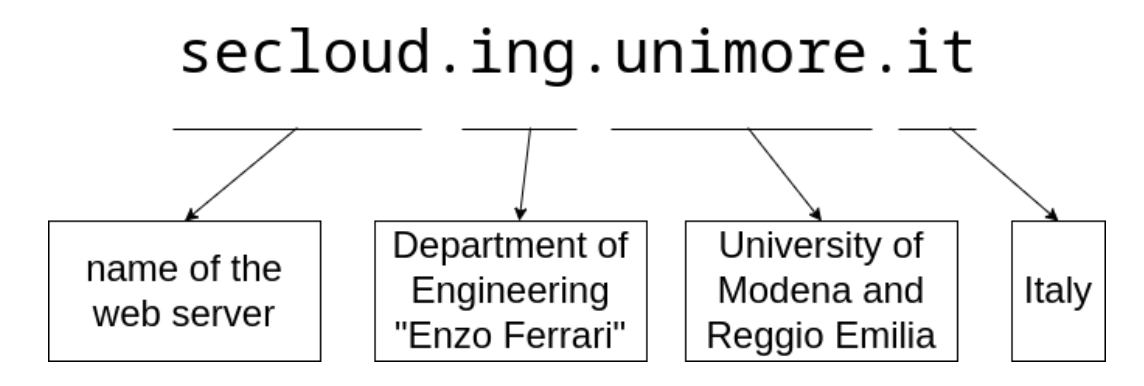
\includegraphics[width=0.6\linewidth]{Images/DNS/hostname.png}
    \caption{Esempio di Hostname canonico.}
\end{figure}

Ogni label rappresenta un livello di gerarchia diverso.
Ovviamente, implementando un sistema di questo tipo, deve essere anche creato un modo per convertire gli hostname nel loro IP e vicevarsa. 

\begin{figure}[!htb]
    \centering
    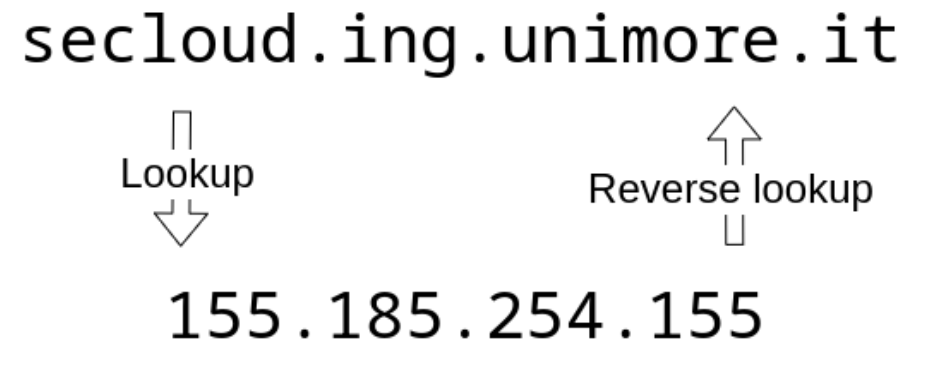
\includegraphics[width=0.4\linewidth]{Images/DNS/lookup.png}
    \caption{Lookup e reverse lookup.}
\end{figure}

All'inizio, venivano usati dei file contenti ogni IP col proprio hostname, ma col crescere dei file si è cercato un modo più scalabile e dinamico, il DNS.

\section{Name Servers}
Divisi in diversi livelli:
\begin{itemize}
    \item \textbf{Root name server:} 13 server, denominati dalla A alla M. Sono distribuiti in ambienti altamente controllati e protetti e gestiti da 12 organizzazioni indipendenti. Inoltre, sono \textbf{autorevole}, devono sapere tutti gli IP dei TLD name server.
    \item \textbf{TLD (Top Level Domain) name server:} deve fornire almeno due name server diversi che siano autorevoli per la sua zona. Tutti conosco gli IP dei SLD name server.
    \item \textbf{SLD (Second Level Domain) name server:} deve fornire almeno due name server diversi che siano autorevoli per la sua zona. Conoscono tutti gli IP dei name server più sotto.
    \item \textbf{Local name server.}
\end{itemize}

\subsection{Resource Records}
In un nameserver, i dati vengono memorizzati come un insieme di \textbf{resources records}. I nameserver consentono meccanismi di ricerca IP diretti e inversi.
Ogni record di risorse ha 6 campi:

\begin{figure}[!htb]
    \centering
    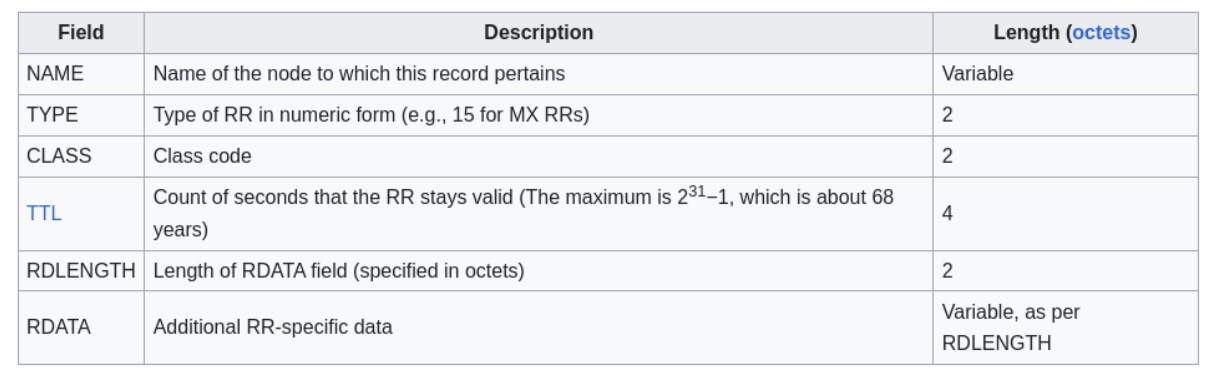
\includegraphics[width=0.8\linewidth]{Images/DNS/Records.png}
    \caption{Campi di un resource record.}
\end{figure}

Alcuni record comuni sono:
\begin{itemize}
    \item \textbf{A:} contiene un indirizzo ipv4 associato a un Fully Qualified Domain Name (FQDN).
    \item \textbf{AAAA:} contiene un indirizzo ipv6 associato a un Fully Qualified Domain Name (FQDN).
    \item \textbf{NS:} memorizza il FQDN del name server autorevole per una determinata zona.
    \item \textbf{NX:} memorizza il FQDN dei server di posta che riceveranno le email per i destinatari di un determinato dominio.
    \item \textbf{CNAME:} contiene il nome canonico di un determinati alias.
    \item \textbf{PRT:} contiene il CNAME associato a un determinati IP.
    \item \textbf{SOA:} contiene parametri di configurazione per la zona.
    \item \textbf{TXT:} associa a una FQDN una stringa arbitraria.
\end{itemize}

Si possono vedere direttamente le query con il comando \textbf{dig}:
\begin{bashbox}
ddig [RR_type] FQDN [@nameserver]
\end{bashbox}
Per esempio:
\begin{bashbox}
ddig A www.unimore.it @8.8.8.8
dig MX unimore.it @155.185.1.2
dig SOA unimore.it @155.155.1.2
dig NS unimore.it @193.0.14.129
\end{bashbox}

\newpage
\subsection{Risoluzione dei nomi in modo distribuito}
Nessun server DNS conosce tutti i valori di tutti i \textbf{record RR} dell'intero Internet, è necessaria una qualche forma di \textbf{cooperazione}.
Il DNS utilizza un approccio client-server:
\begin{enumerate}
    \item Il client avvia il processo di ricerca inviando una query a un name server, di solito si tratta di quello locale configurato in ciascun dispositivo. 
    \item Se conosce la risposta, la fornisce direttamente al client.
    \item Se non conosce la risposta deve chiederla a un altro name server.
\end{enumerate}
Le query possono essere \textbf{ricorsive}, dove ogni name server chiede in automatico a un altro name server, oppure \textbf{iterative} dove sarà l'utente a interrogare più name server.
Ogni name server possiede una cache con alcune risposte, alla scadenza del loro \textbf{TTL} verranno eliminate.

\section{Pacchetto DNS}
Facendo parte del livello applicativo, oltre agli header del protocollo IP e del protocollo UDP, al pacchetto viene aggiunto quello del protocollo DNS.

\begin{figure}[!htb]
    \centering
    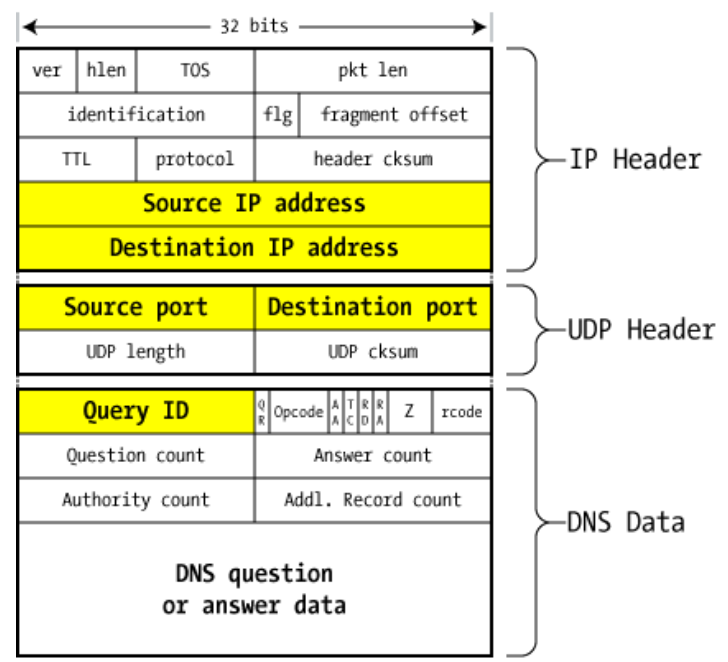
\includegraphics[width=0.5\linewidth]{Images/DNS/Pacchetto_DNS.png}
    \caption{Campi di un resource record.}
\end{figure}

In particolare:
\begin{itemize}
    \item \textbf{Query ID:} identificatore univoco creato nel pacchetto di query e ripetuto dal server nella risposta.
    \item \textbf{QR (Query / Response):} 0 se è una query, 1 se è una risposta.
    \item \textbf{Opcode:} per il tipo di query, standard è 0.
    \item \textbf{AA (Authorative Answer):} 1 se una riposta è autorevole.
    \item \textbf{TC (Trunkated):} la riposta non stava nel pacchetto UDP, sarà necessario fare una nuova richiesta con un segmento TCP.
    \item \textbf{RD (Recursion Desired):} 1 se si vuole fare una query ricorsiva, 0 altrimenti.
    \item \textbf{RA (Recursion Available):} 1 se si può fare una query ricorsiva, 0 altrimenti.
    \item \textbf{Z:} non usato, deve essere 0.
    \item \textbf{rcode:} codice di riposta del server, successo o fallimento.
    \item \textbf{Question record count.} 
    \item \textbf{Answer/Authorative/Additional record count:} inseriti dal server.
    \item \textbf{NDS question:} campo che contiene i dati della richiesta/risposta.
\end{itemize}

\chapter{Esercizi}
\section{Creare un rete}
\begin{figure}[!htb]
    \centering
    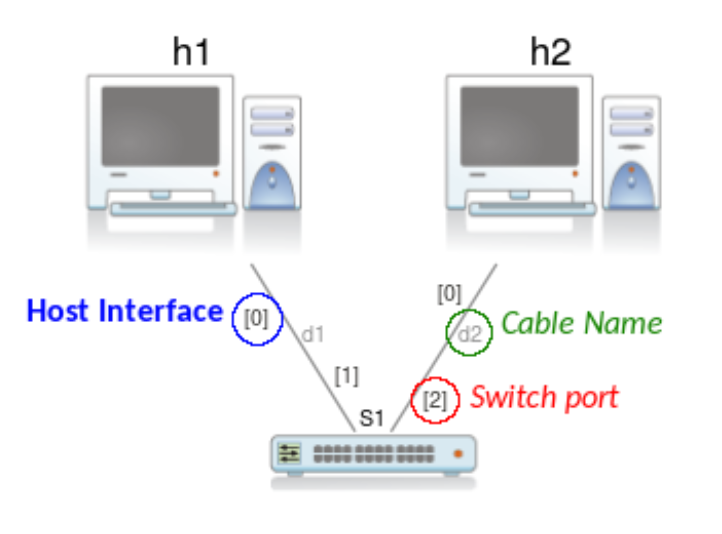
\includegraphics[width=0.4\linewidth]{Images/Esercizi/Marionet.png}
    \caption{Esempio di una rete in Marionet.}
\end{figure}

In Marionet ci sono due tipolgie di cavi:
\begin{enumerate}
    \item \textbf{Cavi crossover:} per connettere macchine sullo stesso livello dello stack.
    \item \textbf{Cavi normali:} per connettere macchine su livelli diversi dello stack.
\end{enumerate}


\end{document}
